\documentclass[preprint,12pt]{elsarticle}

\usepackage{amssymb}
\usepackage{amsmath}
\IfFileExists{booktabs.sty}{\usepackage{booktabs}}{\newcommand{\toprule}{\hline}\newcommand{\midrule}{\hline}\newcommand{\bottomrule}{\hline}}
\usepackage{graphicx}
\usepackage{array}
\usepackage{longtable}
\usepackage{url}
\emergencystretch=2em

\begin{document}
\renewcommand{\thetable}{S\arabic{table}}

\begin{center}
{\Large Supplementary Material}\\[0.5em]
{\large From Identity Exposure to Selective Cross-Domain Calibration of Audit-Risk Probabilities in EEG Emotion Recognition}
\end{center}

\section{Scope and claim boundary}

This supplement documents the complete development and protocol chain for DCS-OPCT v11. The transported quantity is the probability of a configuration-level material identity-optimism event from a frozen audit-risk model. It is not an EEG emotion probability, and the calibration action is not applied to an emotion classifier. EPPVR, CASE, CEAP, SEED-IV, and DREAMER are retrospective development domains for v11. The completed AVDOS-VR PPG and FACED common-montage EEG analyses are post-access exploratory and do not restore either unsuccessful registered confirmation branch. EEGEmotions-27 is a separate pre-signal external robustness test conducted after repository-structure metadata disclosure; it is outside the AMIGOS/Emognition prospective family and returned identity before target outcomes entered action selection. EKM-ED is a prospectively reserved, checksum-verified, implementation-locked attempt that failed the frozen structural endpoint before model fitting; this is non-estimability, not an effectiveness or safety result.

\section{Endpoint ontology and EPPVR acquisition trace}

The task labels used to construct the counterfactual experiments are heterogeneous by design. Participant-experienced dimensional ratings were used in DEAP, MAHNOB-HCI, EPPVR, CASE, CEAP, DREAMER, and EKM-ED, with fixed but dataset-specific cut points. SEED-IV used prespecified extreme stimulus-category contrasts; AVDOS-VR used the official segment-category arousal mapping; FACED and EEGEmotions-27 used stimulus-category polarity; and the reserved AMIGOS protocol uses intended stimulus quadrants. EKM-ED and Emognition reserve participant-experienced SAM valence and arousal with ratings 6--9 high, 1--4 low, and midpoint 5 excluded. These ontologies are not declared equivalent. They are connected only through the higher-level operational endpoint: whether the local identity-dose experiment produces at least 0.02 balanced-accuracy amplification.

\begingroup
\small
\setlength{\tabcolsep}{3pt}
\renewcommand{\arraystretch}{1.08}
\begin{longtable}{@{}>{\raggedright\arraybackslash}p{2.65cm}>{\raggedright\arraybackslash}p{2.85cm}>{\raggedright\arraybackslash}p{3.20cm}>{\raggedright\arraybackslash}p{\dimexpr\textwidth-8.70cm-6\tabcolsep\relax}@{}}
\caption{Dataset-specific endpoint harmonization. Rules and boundaries are fixed within each dataset; semantic differences are recorded without asserting construct equivalence. AMIGOS and Emognition are protocol-only because participant archives remain unavailable; EKM-ED completed a locked attempt but failed structural eligibility before model fitting.}\label{tab:endpoint-harmonization}\\
\toprule
Dataset & Endpoint and ontology & Fixed mapping & Comparability boundary \\
\midrule
\endfirsthead
\multicolumn{4}{@{}l}{\tablename\ \thetable\ continued}\\
\toprule
Dataset & Endpoint and ontology & Fixed mapping & Comparability boundary \\
\midrule
\endhead
\midrule
\multicolumn{4}{r@{}}{Continued on next page}\\
\endfoot
\bottomrule
\endlastfoot
DEAP & arousal/valence; participant self-report & score >= 5 is high; score < 5 is low & Participant-reported dimensional affect; dataset-specific scales and cut points do not make scores metrically interchangeable. \\
MAHNOB-HCI & arousal/valence; participant self-report & score >= 5 is high; score < 5 is low & Participant-reported dimensional affect; dataset-specific scales and cut points do not make scores metrically interchangeable. \\
EPPVR & arousal/valence; participant self-report & score >= 5 is high; score < 5 is low & Participant-reported dimensional affect; dataset-specific scales and cut points do not make scores metrically interchangeable. Label column 3 is dominance and is not analyzed. \\
CASE & arousal/valence; participant annotation/self-report & score >= 5 is high; score < 5 is low & Participant-reported dimensional affect; dataset-specific scales and cut points do not make scores metrically interchangeable. \\
CEAP-360VR & arousal/valence; participant annotation/self-report & score >= 5 is high; score < 5 is low & Participant-reported dimensional affect; dataset-specific scales and cut points do not make scores metrically interchangeable. \\
SEED-IV & valence; fixed stimulus category & happy vs sad & Category contrast is not participant-experienced valence. \\
SEED-IV & arousal; fixed stimulus category & fear vs neutral & Category contrast is not participant-experienced arousal. \\
DREAMER & arousal/valence; participant self-report & rating > 3 is high; rating <= 3 is low & Participant-reported dimensional affect; dataset-specific scales and cut points do not make scores metrically interchangeable. \\
AVDOS-VR & arousal; fixed segment category & Neutral=0; Negative=1; Positive=1 & Segment-category arousal is not a 1-9 participant-experienced rating. \\
FACED & category polarity; fixed stimulus category & amusement, inspiration, joy, or tenderness vs anger, disgust, fear, or sadness & Stimulus polarity is not participant-experienced valence or arousal. \\
EEGEmotions-27 & category polarity; fixed stimulus category with strong self-reported elicitation & 4 prototypical positive IDs vs 6 prototypical negative IDs & Category polarity is not participant-experienced valence or arousal; identity fallback is non-intervention. \\
EKM-ED & valence/arousal; participant self-report & SAM 6--9 high; 1--4 low; 5 excluded & The ontology is participant-experienced affect, but the frozen three-key-window endpoint was structurally non-estimable before model fitting. \\
AMIGOS & valence/arousal; fixed intended stimulus quadrant & published 8/8 high-low short-video quadrants & Intended stimulus quadrant is not participant-experienced affect; no participant result exists. \\
Emognition & valence/arousal; participant self-report & SAM 6-9 high; 1-4 low; 5 excluded & Construct name aligns with dimensional affect, but its scale/exclusion rule is dataset specific; no result exists. \\
\end{longtable}

\endgroup

The local EPPVR source contains 30 byte-matched participant files in both the project dataset directory and the archived handover directory. Each file contains 14 trials with arrays shaped $14\times10\times7000$ and labels shaped $14\times3$. The processing chain identifies channels 0 and 1 as FP1 and FP2, channels 2--4 as GSR/EDA, PPG/BVP, and SKT/HST, and uses 100 Hz. Author-supplied acquisition records identify channels 5--9 collectively as two EOG channels, one PPG channel, one GSR channel, and one temperature channel; their exact within-block order could not be recovered from the inspected acquisition and analysis records and is not required by the executed analysis. The first 1,000 samples form a 10-s baseline and the remaining 6,000 samples form 60 s of post-baseline recording. The three label columns are valence, arousal, and dominance. Only valence and arousal enter the executed analysis, with scores at least 5 assigned to the high class. The head-mounted display was a DPVR E4 and the EEG acquisition front end was ADS1299 based; both the reference and ground electrodes were placed at the right ear. The EPPVR protocol was approved by the Ethical Committee of the University of Electronic Science and Technology of China (approval no. 106142023122227999). Written informed consent and authorization for secondary analysis were obtained.

This trace is deliberately fail-closed. Channels 5--9 and the dominance label are recorded for completeness but excluded from the present analysis. The signal contract itself does not establish acquisition or governance metadata; the device, channel-content, electrode, label, ethics, consent, and secondary-analysis details above are based on author-supplied study records. EPPVR also has one session per participant and no verified cross-participant physical-stimulus identifier, so only the subject axis is admissible and trial position cannot be repurposed as shared stimulus identity.

\section{Counterfactual identity-dose contract}

For every dataset, task, axis, split seed, and crossed test cell, the intervention replaced a fixed class-matched control sub-block with an identity-complete real-row block. Five nominal doses were evaluated. The construction required identical test rows, total training size, binary class counts, and test-identity coverage across dose conditions, with zero train--test row overlap.

The exposure effect, dose-induced amplification, and binary target were
\begin{align}
E_{c,d}&=\operatorname{BAcc}^{\mathrm{exposed}}_{c,d}-\operatorname{BAcc}^{\mathrm{control}}_c,\\
A_{c,d}&=E_{c,d}-E_{c,0},\\
Y_{c,d}&=\mathbb{1}(A_{c,d}\geq0.02).
\end{align}
Dose zero was retained as an anchor and excluded from risk-model outcomes. The primary risk-learning table contained 480 nonzero-dose subject-axis configurations from DEAP and MAHNOB-HCI.

\section{Frozen risk model}

The primary model was L2 logistic regression with $C=0.1$. Continuous predictors were standardized within the training fold. No categorical identities were included.

\begin{table}[h]
\centering
\caption{Frozen audit-risk predictors and full-data standardized coefficients. Coefficients are descriptive because admissibility was based on leave-dataset-out predictions.}
\small
\begin{tabular}{lr}
\toprule
Predictor & Coefficient \\
\midrule
Metadata-prior opportunity & 0.562 \\
Identity-probe encoding margin & 0.286 \\
Model capacity & 0.232 \\
Opportunity change from dose zero & 0.219 \\
Opportunity-change $\times$ encoding margin & 0.211 \\
\bottomrule
\end{tabular}
\end{table}

Dataset identity, row count, participant count, repeated-unit count, task identity, representation identity, and model identity were forbidden. The final model checksum was \texttt{4a9a128b7a2966e1d9f30021f81361a2}\allowbreak\texttt{fb8688920d24a123240ba77795b741b9}.

\begin{table*}[h]
\centering
\caption{Leave-dataset-out public-data validation of the frozen risk model. AP lift is average precision divided by event prevalence.}
\small
\begin{tabular}{lrrrrrr}
\toprule
Held-out dataset & $n$ & Events & AUROC & AP lift & Brier skill & BAcc \\
\midrule
DEAP & 240 & 41 & 0.698 & 2.414 & 0.100 & 0.607 \\
MAHNOB-HCI & 240 & 73 & 0.735 & 1.693 & 0.123 & 0.619 \\
\bottomrule
\end{tabular}
\end{table*}

The locked EPPVR evaluation contained 320 nonzero-dose configurations and 52 material events. AUROC was 0.6658 and AP lift was 2.1921, but Brier skill was $-0.1276$ and balanced accuracy at the frozen threshold was 0.5992. The complete external gate failed. This supports transported ranking only, not transported probabilities or a universal operating threshold.

\section{Post-hoc material-event threshold robustness}

The 0.02 balanced-accuracy endpoint was frozen before EPPVR evaluation and remained unchanged in DCS-OPCT v11. To determine whether the development result depended on an isolated cutoff, we performed a post-hoc sensitivity analysis at 0.010, 0.015, 0.020, 0.025, and 0.030. For each cutoff, the same 480 development configurations were relabeled and the same five-predictor logistic model was refitted under leave-dataset-out validation. Decision thresholds were selected from training folds only. Confidence intervals used 5,000 bootstrap repetitions over complete task-by-representation-by-model-by-split-seed clusters. No external outcome, v11 gate, or frozen decision was recomputed.

\begin{table*}[h]
\centering
\caption{Post-hoc robustness of the operational material-event threshold. Metric entries are minima across the two leave-dataset-out tests. AP lift is average precision divided by event prevalence. The descriptive floors were AUROC $\geq0.65$, AP lift $\geq1.5$, Brier skill $>0$, balanced accuracy $\geq0.60$, and at least 20 events per held-out dataset.}
\small
\textbf{A. Event support and discrimination}\\[0.25em]
\begin{tabular}{crrrr}
\toprule
Threshold & DEAP events & MAHNOB events & Min. AUROC & Min. AP lift \\
\midrule
0.010 & 120 & 114 & 0.575 & 1.165 \\
0.015 & 74 & 91 & 0.632 & 1.429 \\
0.020 & 41 & 73 & 0.698 & 1.693 \\
0.025 & 20 & 56 & 0.677 & 1.709 \\
0.030 & 8 & 40 & 0.754 & 1.906 \\
\bottomrule
\end{tabular}
\\[0.8em]
\textbf{B. Probability and operating-point performance}\\[0.25em]
\begin{tabular}{crrc}
\toprule
Threshold & Min. Brier skill & Min. BAcc & Status \\
\midrule
0.010 & $-0.028$ & 0.533 & Metric fail \\
0.015 & 0.054 & 0.597 & Metric fail \\
0.020 & 0.100 & 0.607 & Supported \\
0.025 & 0.055 & 0.620 & Supported \\
0.030 & 0.091 & 0.664 & Count fail \\
\bottomrule
\end{tabular}
\end{table*}

\begin{figure*}[h]
\centering
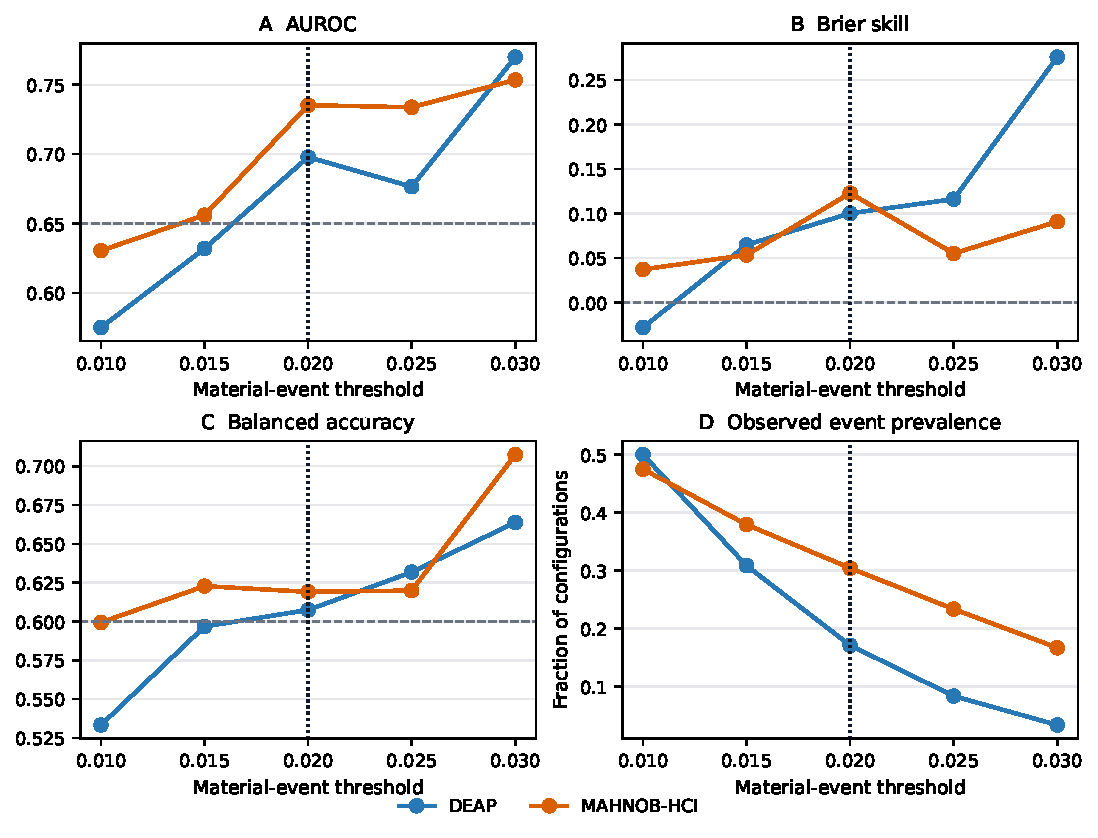
\includegraphics[width=\textwidth]{figures/fig_material_event_threshold_robustness.pdf}
\caption{Post-hoc material-event threshold robustness. The vertical dotted line marks the frozen 0.02 endpoint; horizontal dashed lines mark the descriptive metric floors. Thresholds 0.02 and 0.025 met all four transfer floors and retained at least 20 events in each held-out dataset. The apparent performance increase at 0.03 coincided with only eight DEAP events and was not treated as stronger evidence.}
\end{figure*}

The event definitions at 0.02 and 0.025 agreed for 92.1\% of configurations (Cohen's $\kappa=0.753$; event Jaccard index 0.667). Relative to the 0.02 fits, coefficient-vector cosine similarity at 0.025 was 0.983 for held-out DEAP and 0.993 for held-out MAHNOB-HCI, with complete coefficient-sign agreement. The frozen 0.02 result was numerically reproduced with maximum absolute discrepancy $2.22\times10^{-16}$. These findings place 0.02 at the lower edge of a bounded operational region; they do not optimize the endpoint, validate physiological materiality, or expand the external-effectiveness claim.

\section{Post-hoc engineering anchor, cluster dependence, and audit yield}

We first evaluated whether a distortion of 0.02 balanced accuracy is large relative to model-selection margins. Under the joint-unseen reference protocol, each dataset--task--seed unit contained four candidate models. We computed the top-two margin and all six absolute pairwise margins. Seventeen of 20 top-two margins (85\%, cluster-bootstrap 95\% CI 70--100\%) and 65 of 120 pairwise margins (54.2\%, 44.2--65.0\%) were no greater than 0.02. This anchors the endpoint to model-selection sensitivity without assigning it physiological or clinical meaning.

The earlier row-ranked audit diagnostic could split the four nonzero doses belonging to one configuration cluster. We therefore repeated the allocation at the unit used by the v11 certificate: dataset--task--representation--model--split seed, with all four dose configurations selected together. Within each held-out source dataset, the frozen cluster score was the maximum of its four leave-dataset-out risk probabilities. Budgets of 10--50\% selected the same fraction of complete clusters from each dataset. The primary reporting cell was designated post hoc at the frozen 0.02 event threshold and the existing 20\% minimum-budget condition; other cells were sensitivity analyses. Random allocation retained the same per-dataset cluster counts. An outcome-informed oracle is shown only as a descriptive ceiling.

At the designated cell, 24 of 120 clusters were selected, requiring 96 configuration labels. Frozen ranking captured 19 of 56 event-bearing clusters (33.9\%), compared with a random mean of 20.0\% and a random 97.5th percentile of 28.6\%. The descriptive one-sided stratified hypergeometric probability of capturing at least 19 event-bearing clusters was $p=0.000345$. The selected clusters contained 43 of 114 material-event configurations (37.7\%) and 37.4\% of total amplification above the 0.02 threshold. Maximum, mean, and median aggregation of the four frozen per-dose probabilities selected exactly the same 24 clusters (all pairwise Jaccard indices 1.0) and therefore produced identical yield estimates.

The four dose rows were not statistically independent. At the primary threshold, overall ICC(1,1) was 0.420 for the binary material event, 0.591 for amplification, and 0.753 for the frozen risk probability. The corresponding design-effect-based effective row counts were approximately 212, 173, and 147 rather than 480. Complete-cluster bootstrap intervals were 1.30--1.75 times as wide as naive row-bootstrap intervals across event prevalence and mean amplification in the pooled and dataset-specific analyses. All inferential summaries therefore retain the complete cluster as the resampling unit.

\begin{table}[!htbp]
\centering
\caption{Designated complete-cluster audit-yield and dependence results. The post-hoc reporting cell used the frozen 0.02 event threshold and the existing 20\% minimum-budget condition.}
\label{tab:complete-cluster-audit-yield}
\small
\resizebox{\textwidth}{!}{\begin{tabular}{@{}lrr@{}}
\toprule
Quantity & Estimate & Comparator or consequence \\
\midrule
Event-bearing clusters captured & 0.339 & Random mean 0.200 \\
Exact stratified random-allocation test & $p=0.0003$ & One-sided, post-hoc designated cell \\
Event configurations captured & 0.377 & 43/114 configurations \\
Material excess captured & 0.374 & Above the 0.02 endpoint \\
Material-event ICC(1,1) & 0.420 & Effective $n=212$ of 480 \\
Amplification ICC(1,1) & 0.591 & Effective $n=173$ of 480 \\
\bottomrule
\end{tabular}
}
\end{table}

\begin{figure*}[!htbp]
\centering
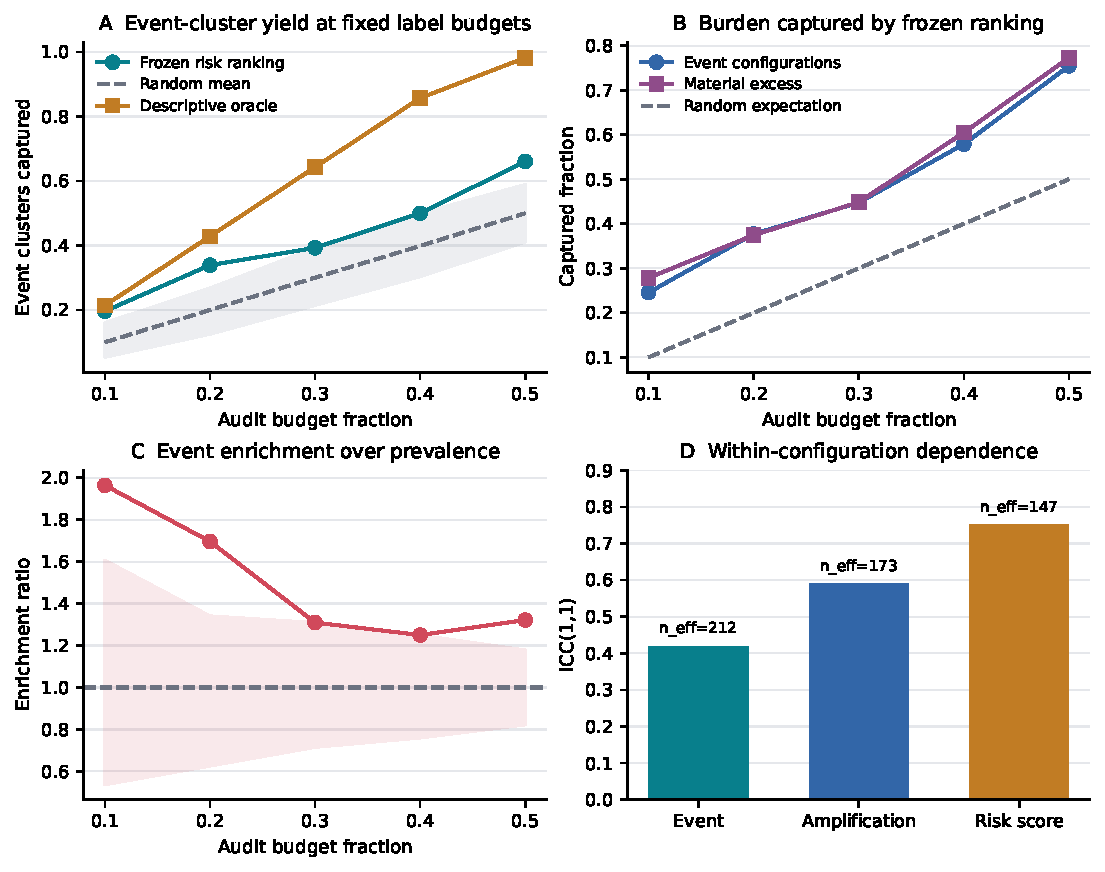
\includegraphics[width=0.92\textwidth]{figures/fig_cluster_dependence_audit_yield.pdf}
\caption{Complete-cluster audit allocation and dependence sensitivity. (A) Frozen risk ranking, same-budget random allocation, and an outcome-informed descriptive oracle for event-bearing-cluster capture. Shading is the central 95\% random-allocation interval. (B) Event configurations and material excess captured by the frozen ranking. (C) Enrichment of selected event-bearing clusters over prevalence. (D) ICC(1,1) and design-effect-based effective row counts at the frozen 0.02 threshold. These are retrospective source-domain diagnostics, not prospective workflow-utility or external-effectiveness results.}
\label{fig:complete-cluster-audit-yield}
\end{figure*}

The exact primary comparison shows that the frozen Stage II ranking concentrated audit yield after respecting the complete-cluster label unit. It does not establish causal component necessity, measured cost effectiveness, external effectiveness, or a transferable operating-point guarantee. The binary decision-curve results from the earlier row-level diagnostic are retained as exploratory provenance but are not used for the complete-cluster primary claim.

\section{Higher-level dataset--task--seed sensitivity}

The complete-configuration analysis retains all four doses together but representations and models within a dataset--task--seed family still share source trials, labels, and data partitions. We therefore repeated the primary 0.02-threshold, 20\% budget analysis using dataset--task--seed as the indivisible unit. The two source datasets contributed ten blocks each (two tasks by five split seeds), and every block contained 24 rows spanning three representations, two models, and four nonzero doses. Two whole blocks were selected per dataset, preserving the same 96-row label budget as the complete-configuration analysis.

Maximum, mean, and median aggregation of the frozen risk probability selected the same four blocks. They captured 26.3\% of all material-event rows and 25.9\% of material excess, with event prevalence 1.316 times the source-domain average. We enumerated all $\binom{10}{2}^2=2{,}025$ valid stratified same-budget allocations. The exact one-sided probabilities were $p=0.207$ for event-row sensitivity and $p=0.260$ for material-excess capture. The higher-level result therefore did not provide statistically persuasive evidence that the frozen ordering improves whole-block audit yield.

Stratified bootstrap resampling of the 20 blocks gave event prevalence 0.238 (95\% interval 0.165--0.310) and mean amplification 0.0107 (0.0071--0.0140). These intervals account for shared representation, model, dose, trial, and split structure within each dataset--task--seed family, but remain conditional on only two source datasets. They neither create domain-level replication nor support prospective workflow utility.

\begin{table}[!htbp]
\centering
\caption{Post-hoc higher-level dependence sensitivity at the frozen 0.02 endpoint and 20\% budget. Exact probabilities enumerate all stratified whole-block allocations.}
\label{tab:higher-level-cluster}
\small
\resizebox{\textwidth}{!}{\begin{tabular}{@{}lr@{}}
\toprule
Quantity & Estimate \\
\midrule
Higher-level units & 20 dataset--task--seed blocks \\
Selected units at 20\% budget & 4 blocks / 96 rows \\
Event rows captured & 0.263 \\
Material excess captured & 0.259 \\
Event enrichment & 1.316 \\
Exact random-allocation $p$, event capture & 0.207 \\
Exact random-allocation $p$, excess capture & 0.260 \\
Event prevalence, 95\% block-bootstrap interval & 0.237 [0.165, 0.310] \\
Mean amplification, 95\% block-bootstrap interval & 0.0107 [0.0071, 0.0140] \\
\bottomrule
\end{tabular}
}
\end{table}

\begin{figure*}[!htbp]
\centering
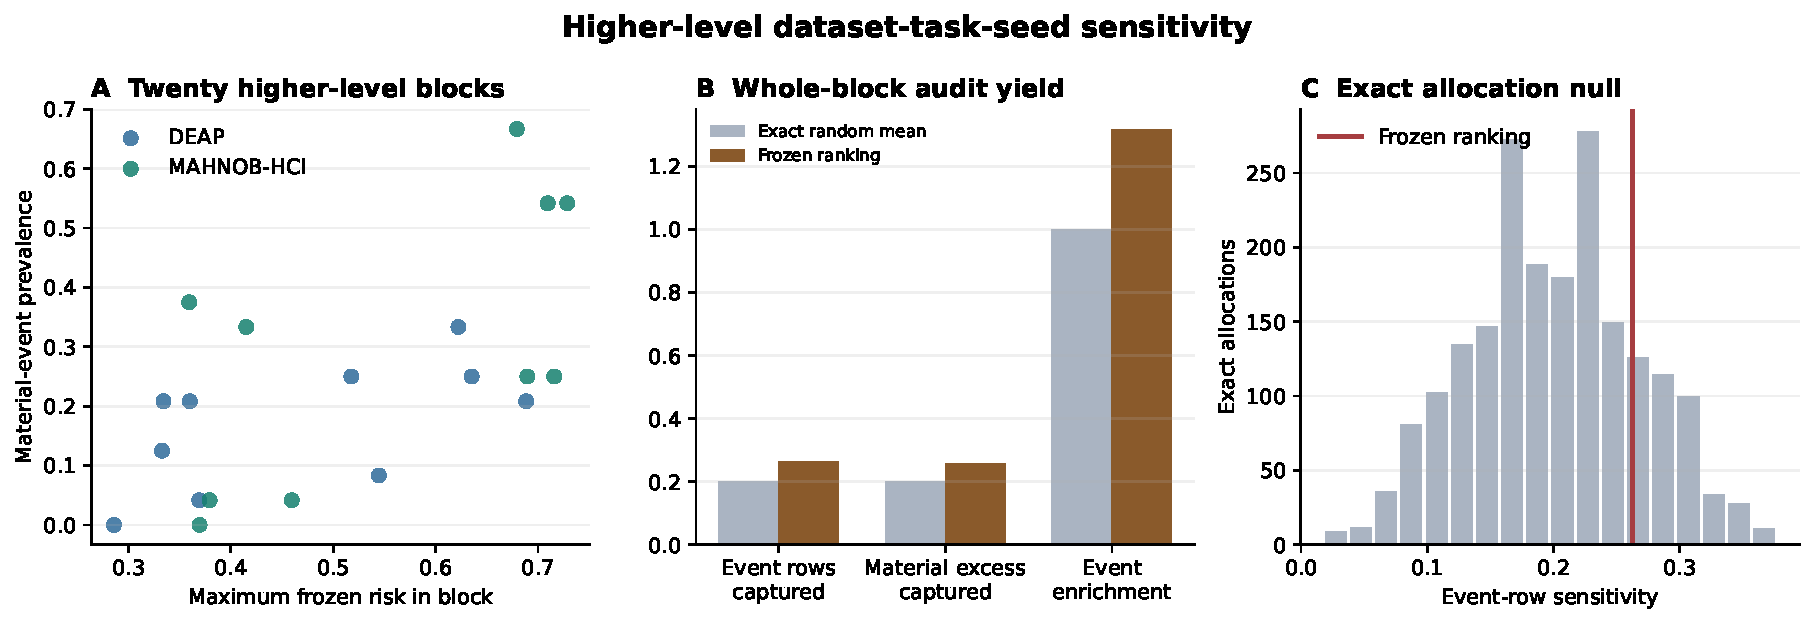
\includegraphics[width=0.96\textwidth]{figures/fig_higher_level_cluster_sensitivity.pdf}
\caption{Dataset--task--seed sensitivity. (A) Frozen block risk versus material-event prevalence for the 20 higher-level units. (B) Whole-block frozen-risk allocation compared with the exact random-allocation mean. (C) Exact null distribution for event-row sensitivity; the vertical line is the frozen allocation. The result is conditional post-hoc sensitivity, not independent-domain validation.}
\label{fig:higher-level-cluster}
\end{figure*}

\section{Model-ranking consequences}

\begin{table*}[h]
\centering
\caption{Selected model-ranking consequences under subject exposure. Rates are proportions across five split seeds. Regret is joint-unseen balanced accuracy.}
\small
\resizebox{\textwidth}{!}{%
\begin{tabular}{llrrrr}
\toprule
Dataset & Task & Winner changed & Material reversal & Mean regret & Pairwise inversion \\
\midrule
DEAP & Arousal & 0.80 & 0.60 & 0.0212 & 0.733 \\
DEAP & Valence & 1.00 & 0.40 & 0.0205 & 0.753 \\
MAHNOB-HCI & Arousal & 0.80 & 0.60 & 0.0229 & 0.480 \\
MAHNOB-HCI & Valence & 0.60 & 0.40 & 0.0145 & 0.380 \\
\bottomrule
\end{tabular}
}
\end{table*}

These values quantify a model-selection consequence, not a physiological effect. A material reversal means that the exposed protocol selected a different candidate and that this choice lost practically relevant joint-unseen performance.

\section{DCS-OPCT fixed gates}

The CORAL and quantile components were separately projected by $T_{a,b}(p)=\sigma(a\operatorname{logit}(p)+b)$ with $a>0$. Parameters were optimized for 500 epochs on CUDA with learning rate 0.03 and regularization $10^{-4}$. The scale range was 0.1--5.0 and the absolute shift limit was 5.0. A component required absolute probability mean shift at most 0.10, rank at least 0.999999, and zero order inversions.

The witness required directional agreement at least 0.90, displacement cosine at least 0.90, and normalized disagreement at most 0.35. Failure of any rule returned identity before labeled certification.

\begingroup
\scriptsize
\setlength{\tabcolsep}{3pt}
\renewcommand{\arraystretch}{1.02}
\begin{longtable}{>{\raggedright\arraybackslash}p{0.17\textwidth}>{\raggedright\arraybackslash}p{0.13\textwidth}>{\raggedright\arraybackslash}p{0.25\textwidth}>{\raggedright\arraybackslash}p{0.33\textwidth}}
\caption{Provenance and inferential role of frozen endpoints, applicability gates, and release criteria. Frozen means fixed before the relevant target action or held-out evaluation; it does not imply independent optimality. Post-hoc stability analyses described decision margins only and did not select these values.}
\label{tab:threshold-provenance}\\
\toprule
Quantity & Value & Provenance & Inferential role and boundary \\
\midrule
\endfirsthead
\multicolumn{4}{l}{\footnotesize\itshape Table~\thetable\ continued from previous page}\\
\toprule
Quantity & Value & Provenance & Inferential role and boundary \\
\midrule
\endhead
\midrule
\multicolumn{4}{r}{\footnotesize Continued on next page}\\
\endfoot
\bottomrule
\endlastfoot
Material optimism endpoint & 0.02 BAcc & Operational endpoint frozen before EPPVR evaluation & Defines $Y_{c,d}$; not a physiological or clinical threshold and not independently optimal \\
Risk operating threshold & 0.18619 & Selected from training-only out-of-fold predictions and frozen before EPPVR & Converts frozen risk probabilities to an audit flag; target outcomes did not select it \\
Component mean displacement & $\leq0.10$ & Fixed v11 applicability constraint before external action use & Fail-closed bound on probability movement; local post-hoc perturbations do not validate optimality \\
Rank agreement & $\geq0.999999$ & Numerical verification tolerance & Confirms near-exact rank preservation; not an empirical performance threshold \\
Order inversions & 0 & Structural implementation requirement & Any inversion makes the probability action ineligible \\
Directional agreement & $\geq0.90$ & Fixed v11 witness criterion before external action use & Requires concordant component directions; heuristic applicability bound, not an identified causal cutoff \\
Displacement cosine & $\geq0.90$ & Fixed v11 witness criterion before external action use & Requires global directional similarity between independently constructed components \\
Normalized disagreement & $\leq0.35$ & Fixed v11 witness criterion before external action use & Limits component-wise disagreement; not optimized on external effectiveness \\
Brier-gain lower bound & $>0.001$ & Fixed release-certificate requirement before held-out evaluation & Requires positive one-sided certified calibration gain for the registered action \\
AUROC noninferiority & $\geq-0.02$ & Fixed release constraint before held-out evaluation & Prevents a released calibration map from materially degrading ranking \\
Material negative transfer & $<-0.001$ gain & Prespecified retrospective decision-analysis endpoint & Defines a released-action adverse event; zero observed events does not prove future-domain non-harm \\
\end{longtable}
\endgroup

\section{Distribution-covered certificate}

Each complete cluster contained the four nonzero doses for one task, representation, model, and split seed. Seven unlabeled geometry summaries described the identity probability, candidate probability, their displacement, and the 0.5 decision-flip fraction. Within every task-by-representation-by-model stratum, all admissible two-cluster or three-cluster audit subsets were enumerated. The selected subset minimized squared mismatch in standardized means plus 0.05 times squared mismatch in standardized standard deviations. The parity rule produced 40 audit and 40 held-out clusters for each 320-row domain.

Brier gain was estimated with 5,000 bootstrap repetitions, resampling complete clusters within strata. The one-sided familywise lower confidence bound had to exceed 0.001. AUROC noninferiority used margin $-0.02$ and was certified analytically only after exact order preservation was verified.

\section{Preserved predecessor failures}

The final method was not the first attempted transport rule. All predecessor outcomes remain in the reproducibility archive and constrain interpretation of v11.

\begin{table*}[h]
\centering
\caption{Preserved development failures and the change they motivated.}
\small
\resizebox{\textwidth}{!}{%
\begin{tabular}{llll}
\toprule
Version & Preserved outcome & Diagnosis & Consequence for v11 \\
\midrule
v6 & CEAP external effectiveness failure & Positive certificate did not reproduce & External gain required \\
v7 & CEAP release/effect failure & Consensus did not repair weak support & Identity fallback retained \\
v8 & Development-gate failure & Equal component averaging was unstable & Primary and witness roles separated \\
v9 & CEAP release rate 0.39 & Random half-audits had weak coverage & Distribution-covered audit introduced \\
v10 & Released negative transfer & Stronger correction exceeded safe benefit & v9 probability action restored unchanged \\
\bottomrule
\end{tabular}
}
\end{table*}

The v11 change was therefore confined to audit allocation. It did not amplify the v9 correction, weaken any applicability threshold, or lower the Brier-gain requirement.

\begin{figure}[h]
\centering
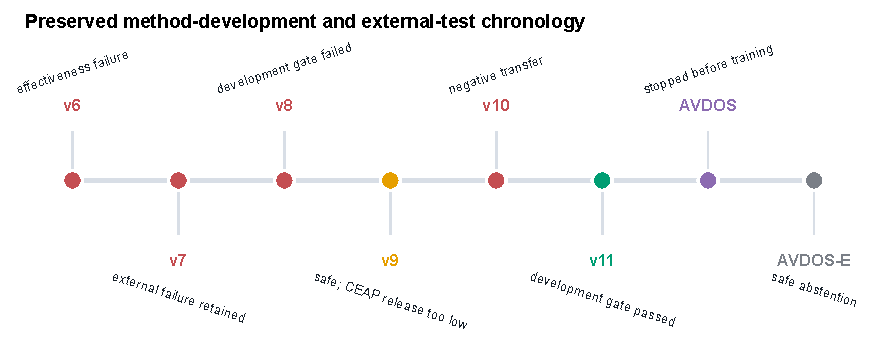
\includegraphics[width=\textwidth]{figures/fig_v11_failure_and_protocol_timeline.pdf}
\caption{Chronology of method failures, v11 freeze, and AVDOS-VR protocol status. Failed branches are retained as evidence and are not reclassified as successful validation.}
\end{figure}

\section{AVDOS-VR protocol and evidence status}

The reserved one-shot AVDOS-VR confirmation did not reach model training. Participant 8 had only two Positive windows for the locked three-block construction, and registered HRV fields contained official $-1$ quality sentinels. No later analysis restores confirmatory status.

The effective post-access exploratory contract used arousal only, with official labels Neutral$=0$ and Negative/Positive$=1$. It contained 37 participants, 222 trials, four PPG-only representations, five split seeds, a linear logistic classifier, and a 40-epoch CUDA MLP. Three implementation defects were recorded and corrected through chronological amendments before the final 3,600-fit run. The base protocol's threshold-5 paragraph is superseded by the later label-semantics records and is not the executed definition.

Raw-PPG identity-probe balanced accuracy was 0.234 for the linear classification and 0.370 for radial-basis classification. Dose-induced effects were non-monotonic. CORAL and quantile OPCT shifts were 0.1509 and 0.3696; both exceeded the 0.10 displacement budget. The method therefore returned identity, giving Brier gain 0 and AUROC change 0 by construction. This is exploratory non-intervention without evidence of external effectiveness.

\section{FACED protocol and evidence status}

The registered FACED branch required a common 32-channel EEG montage and at least 100 eligible participants. File-level and channel-label audits found two acquisition groups: 61 participants had T3/T4, T5/T6, and A1/A2, whereas 62 had T7/T8, P7/P8, and HEOR/HEOL. Relabeling the temporal electrodes was technically defensible, but treating auricular reference channels as horizontal EOG would not be. The largest physiologically comparable EEG montage therefore contained 30 channels, and neither 32-channel subgroup met the registered sample-size requirement. The registered branch was terminated and retained as a structural eligibility failure.

A post-access amendment evaluated the shared 30-channel montage in all 123 participants. Each participant contributed 24 non-neutral video trials, yielding 2,952 participant--video rows. Three representations, two classifiers, five split seeds, five subject folds, and five dose levels produced 4,500 completed fits. Split validation confirmed zero train--test row overlap and complete coverage of test identities. Identity-probe balanced accuracy ranged from 0.8853 to 0.9920 against chance accuracy 0.00813, but dose-induced amplification ranged from $-0.01660$ to 0.01389. None of the 120 nonzero-dose configurations met the frozen 0.02 material-event definition.

CORAL and quantile probability shifts were 0.1224 and 0.3340, both above the frozen 0.10 applicability limit. The action was therefore identity. Both the 60-configuration audit partition and the 60-configuration held-out partition contained zero events, so AUROC and calibration effectiveness were undefined rather than successful. This post-access result supports only the mechanism boundary that strong participant encoding need not produce material utilization at the frozen endpoint. It does not support external calibration effectiveness or a general safety claim.

\begin{figure*}[h]
\centering
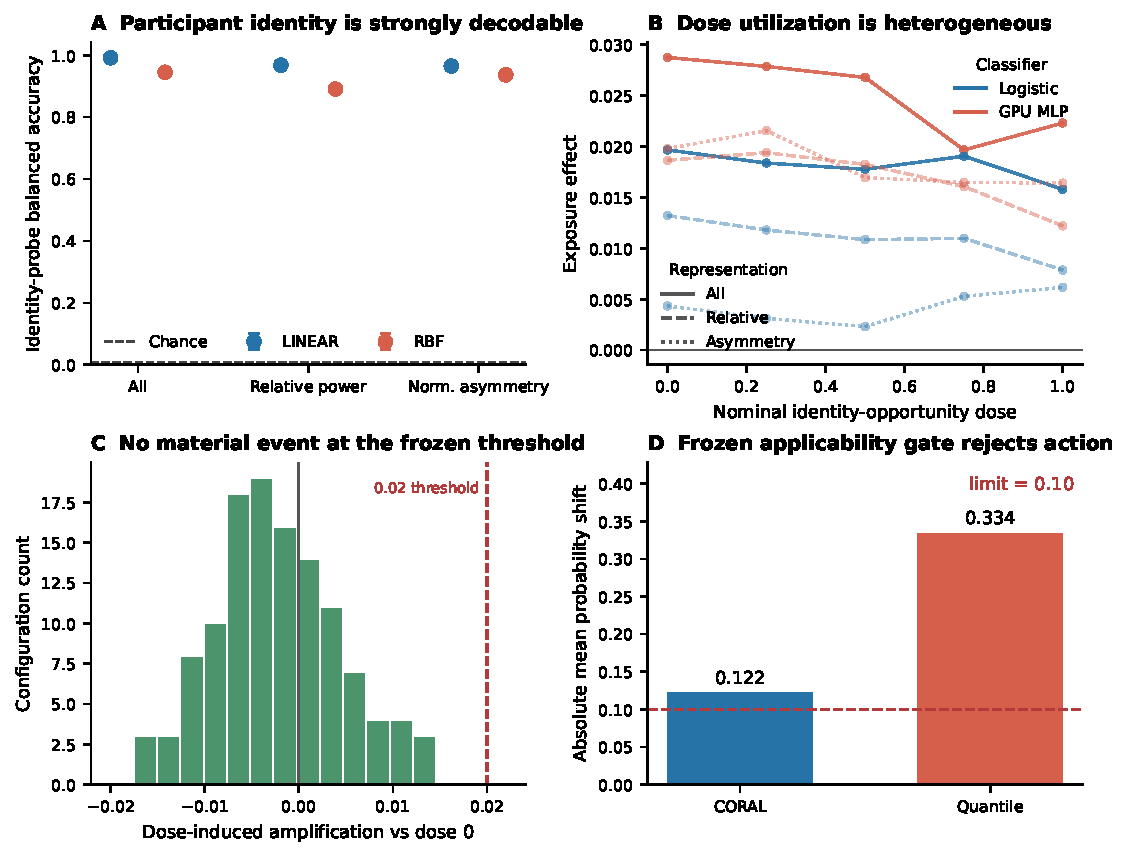
\includegraphics[width=\textwidth]{figures/fig_faced_post_access_external_boundary.pdf}
\caption{Post-access exploratory FACED common-montage analysis. Strong participant identity encoding coexisted with small heterogeneous dose effects, zero material events, and failure of both frozen component-displacement gates.}
\end{figure*}

\begin{table*}[h]
\centering
\caption{FACED post-access exploratory dose effects by representation and classifier.}
\small
\resizebox{\textwidth}{!}{\begin{tabular}{llrrrr}
\toprule
Representation & Classifier & Mean $\Delta$ & Min $\Delta$ & Max $\Delta$ & Events \\
\midrule
All & GPU MLP & -0.0046 & -0.0166 & 0.0051 & 0/20 \\
All & Logistic & -0.0019 & -0.0115 & 0.0078 & 0/20 \\
Normalized asymmetry & GPU MLP & -0.0019 & -0.0115 & 0.0122 & 0/20 \\
Normalized asymmetry & Logistic & -0.0001 & -0.0112 & 0.0139 & 0/20 \\
Relative power & GPU MLP & -0.0022 & -0.0149 & 0.0102 & 0/20 \\
Relative power & Logistic & -0.0028 & -0.0091 & 0.0071 & 0/20 \\
\bottomrule
\end{tabular}
}
\end{table*}

\section{Matched audit-budget comparator analysis}

The frozen v11 held-out halves were retained unchanged. Within each frozen audit half, 100 balanced cluster orders generated nested 20\%, 40\%, 60\%, 80\%, and 100\% labeled subsets. EPPVR, CASE, and CEAP therefore used 32, 64, 96, 128, and 160 labeled configurations; SEED-IV and DREAMER used 24, 48, 72, 96, and 120. The compared procedures were selective DCS-OPCT, the unconditional DCS candidate as a diagnostic, positive-slope target Platt scaling, target isotonic calibration, monotone beta calibration, temperature scaling, Platt or beta calibration with disjoint fitting and certification subsets, and same-audit two-fold cross-fit-certified Platt or beta calibration. In the cross-fit procedures, each fold was predicted by the map fitted on the opposite fold; the combined out-of-fold predictions were certified over the complete audit set, and a passing method was then refitted on all audit labels for held-out release. The monotone beta map was $\sigma[a\log p-b\log(1-p)+c]$ with $a,b>0$; temperature scaling was $\sigma[s\operatorname{logit}(p)]$ with $s>0$. Parametric calibrators were optimized on CUDA for 1,000 epochs. Every procedure was evaluated on the same frozen held-out half.

Material negative transfer was defined as release with held-out Brier gain below $-0.001$. At the minimum budget, selective DCS-OPCT had zero material-negative events. Direct Platt frequencies were 0.06, 0.69, 0.53, 0.05, and 0.25 for EPPVR, SEED-IV, DREAMER, CASE, and CEAP. Direct beta frequencies were 0.06, 0.69, 0.53, 0.06, and 0.28. Isotonic frequencies were 0.17, 0.99, 0.77, 0.19, and 0.66. Split certification reduced release but did not eliminate material negative transfer: minimum-budget frequencies were 0.00--0.22 for split Platt and 0.02--0.23 for split beta. At the full budget, direct Platt and beta achieved larger mean gain in four domains, showing that the DCS result is a low-label intervention tradeoff rather than calibration superiority.

Table~\ref{tab:strong-low-label} gives an equal-domain descriptive summary over the 20\% and 40\% budget cells. Direct Platt and beta produced the highest mean gains but material-negative frequencies of 0.263 and 0.268. Selective DCS-OPCT had a lower mean gain of 0.0134 and zero material-negative events. The unconditional DCS diagnostic also had zero observed material-negative events because the precomputed action happened to be beneficial in all three applicable development domains and remained identity in the two inapplicable domains; this is a retrospective diagnostic, not a release rule or general safety guarantee.

\begin{center}
\begin{minipage}{\textwidth}
\refstepcounter{table}
\textbf{Table~\thetable:} Equal-domain descriptive summary over the 20\% and 40\% matched audit-budget cells. Mean gain is held-out Brier gain relative to identity. Material negative denotes release with gain below $-0.001$. AUROC failure denotes a released action with AUROC change below $-0.02$.
\label{tab:strong-low-label}
\par\medskip
\centering
\small
\resizebox{\textwidth}{!}{\begin{tabular}{lrrrr}
\toprule
Method & Release rate & Mean gain & Material negative & AUROC failure \\
\midrule
DCS selective & 0.463 & 0.0134 & 0.000 & 0.000 \\
DCS unconditional diagnostic & 0.600 & 0.0166 & 0.000 & 0.000 \\
Target Platt & 1.000 & 0.0181 & 0.263 & 0.000 \\
Target beta & 1.000 & 0.0174 & 0.268 & 0.000 \\
Target temperature & 1.000 & -0.0000 & 0.356 & 0.000 \\
Target isotonic & 1.000 & 0.0072 & 0.497 & 0.221 \\
Split-certified Platt & 0.324 & 0.0077 & 0.070 & 0.000 \\
Split-certified beta & 0.305 & 0.0069 & 0.077 & 0.000 \\
Cross-fit-certified Platt & 0.265 & 0.0081 & 0.060 & 0.000 \\
Cross-fit-certified beta & 0.250 & 0.0077 & 0.057 & 0.000 \\
\bottomrule
\end{tabular}
}
\end{minipage}
\end{center}

\section{Cross-fit certification inference}

At the 20\% budget, cross-fit-certified Platt produced material-negative transfer in 21, 17, and 13 of 100 repetitions in SEED-IV, DREAMER, and CEAP. Cross-fit-certified beta produced 20, 16, and 12 events. No such event was observed for DCS-OPCT. Table~\ref{tab:crossfit-paired} reports paired gain intervals, sign-randomization tests, and exact McNemar tests. Holm correction covered all 150 dataset-by-budget-by-comparator cells. The one-sided 95\% upper bounds for the unobserved DCS event frequency among released actions ranged from 0.0295 to 0.0464, so zero observed events must not be interpreted as zero future risk.

\begin{center}
\begin{minipage}{\textwidth}
\refstepcounter{table}
\textbf{Table~\thetable:} Paired DCS-OPCT minus cross-fit-certified calibration inference at 20\% audit budget. Harm is the comparator material-negative count; DCS had zero events in every row. Confidence intervals used 20,000 paired bootstrap repetitions and randomization tests used 100,000 sign permutations.
\label{tab:crossfit-paired}
\par\medskip
\centering
\small
\resizebox{\textwidth}{!}{\begin{tabular}{llrrrr}
\toprule
Dataset & Cross-fit map & $\Delta$ gain [95\% CI] & $p_{\mathrm{Holm}}$ & Harm & McNemar $p_{\mathrm{Holm}}$ \\
\midrule
EPPVR & Platt & +0.0099 [+0.0070, +0.0129] & 0.0015 & 0/100 & 1.0000 \\
EPPVR & Beta & +0.0109 [+0.0078, +0.0138] & 0.0015 & 0/100 & 1.0000 \\
SEED-IV & Platt & +0.0006 [+0.0003, +0.0010] & 0.0015 & 21/100 & 0.0001 \\
SEED-IV & Beta & +0.0006 [+0.0003, +0.0010] & 0.0015 & 20/100 & 0.0003 \\
DREAMER & Platt & +0.0061 [+0.0028, +0.0100] & 0.0315 & 17/100 & 0.0020 \\
DREAMER & Beta & +0.0059 [+0.0025, +0.0098] & 0.0614 & 16/100 & 0.0039 \\
CASE & Platt & +0.0026 [-0.0049, +0.0102] & 1.0000 & 0/100 & 1.0000 \\
CASE & Beta & +0.0026 [-0.0048, +0.0100] & 1.0000 & 0/100 & 1.0000 \\
CEAP & Platt & +0.0095 [+0.0062, +0.0137] & 0.0015 & 13/100 & 0.0305 \\
CEAP & Beta & +0.0095 [+0.0061, +0.0136] & 0.0015 & 12/100 & 0.0596 \\
\bottomrule
\end{tabular}
}
\end{minipage}
\end{center}

\section{Frozen leave-one-component diagnostics}

We reconstructed the frozen component probabilities on CUDA and required the resulting component diagnostics and action locks to match the archived v11 values before analysis. All counterfactual variants retained the same CORAL candidate, positive-slope OPCT parameters, 0.02 material endpoint, 0.001 Brier certificate threshold, bootstrap seed, distribution-covered audit assignment, and held-out rows. The variants removed only the named decision component and did not refit or retune any gate. Table~\ref{tab:leave-one-component} uses R for a released correction followed by held-out Brier gain, I for rejection by the unlabeled gate, and C-reject for a candidate that reached the labeled audit but failed its unchanged certificate.

\begin{center}
\begin{minipage}{\textwidth}
\refstepcounter{table}
\textbf{Table~\thetable:} Same-assignment leave-one-component diagnostic. Removing the quantile witness made DREAMER audit-eligible; removing the complete unlabeled applicability screen also made SEED-IV audit-eligible. The fixed labeled certificate rejected both candidates. These results diagnose observed component roles and do not establish causal necessity or prospective safety.
\label{tab:leave-one-component}
\par\medskip
\centering
\small
\resizebox{\textwidth}{!}{\begin{tabular}{lccccc}
\toprule
Variant & EPPVR & SEED-IV & DREAMER & CASE & CEAP \\
\midrule
Full v11 & R (+0.0263) & I & I & R (+0.0485) & R (+0.0085) \\
Without quantile witness & R (+0.0263) & I & C-reject & R (+0.0485) & R (+0.0085) \\
Without unlabeled screen & R (+0.0263) & C-reject & C-reject & R (+0.0485) & R (+0.0085) \\
\bottomrule
\end{tabular}
}
\end{minipage}
\end{center}

For DREAMER, witness removal exposed an audit Brier gain of $-0.00047$ with lower bound $-0.00413$. For SEED-IV, removing the complete unlabeled screen exposed a gain of $-0.03146$ with lower bound $-0.04458$. Neither candidate was released. The unchanged certificate therefore acted as a final outcome-based veto, while the unlabeled stages avoided spending labels on candidates that were rejected upstream in full v11.

To isolate audit allocation, we retained the full frozen unlabeled action and certificate but replaced the deterministic distribution-covered assignment with the 100 stored random balanced half-audits from v9. Table~\ref{tab:distribution-coverage-diagnostic} reports release over all repetitions and mean held-out gain with rejected repetitions counted as identity gain zero. EPPVR and CASE were stable, whereas CEAP was certified in only 60\% of random halves. The distribution-covered assignment selected a CEAP half with a positive certificate and held-out gain 0.0085. This is a retrospective stability diagnostic, not evidence that the deterministic assignment is optimal.

\begin{center}
\begin{minipage}{\textwidth}
\refstepcounter{table}
\textbf{Table~\thetable:} Distribution-covered assignment versus 100 stored random balanced half-audits under the unchanged full action and certificate. Covered gain is the v11 held-out Brier gain. Random mean gain includes identity gain zero after certificate rejection; material harm denotes a released gain below $-0.001$.
\label{tab:distribution-coverage-diagnostic}
\par\medskip
\centering
\small
\resizebox{\textwidth}{!}{\begin{tabular}{lrrrr}
\toprule
Dataset & Covered gain & Random release & Random mean gain & Random material harm \\
\midrule
EPPVR & +0.0263 & 0.99 & +0.0237 & 0.00 \\
SEED-IV & +0.0000 & 0.00 & +0.0000 & 0.00 \\
DREAMER & +0.0000 & 0.00 & +0.0000 & 0.00 \\
CASE & +0.0485 & 1.00 & +0.0370 & 0.00 \\
CEAP & +0.0085 & 0.60 & +0.0044 & 0.00 \\
\bottomrule
\end{tabular}
}
\end{minipage}
\end{center}


\section{End-to-end component efficiency under a common label ceiling}

The simplified variants reused the frozen candidate probabilities, distribution-covered assignments, held-out rows, certificates, and 720-configuration action-stage budget ceiling. Risk ranking alone did not define a calibration action. Certificate-only processing sent all 720 labels to the five target-domain certificates. The primary unlabeled component screen reduced this requirement to 600 by stopping SEED-IV, and the complementary witness reduced it to 480 by additionally stopping DREAMER. All three calibration variants released EPPVR, CASE, and CEAP and retained the same summed held-out Brier gain. The resulting 33.3\% reduction is retrospective label-demand accounting under the archived assignment, not a prospective sample-complexity theorem or proof of universal component necessity.

\begin{table}[!htbp]
\centering
\caption{Same-ceiling simplified end-to-end comparator summary. Fraction is the proportion of the 720-configuration ceiling entering action-stage processing.}
\label{tab:simplified-comparators}
\small
\resizebox{\textwidth}{!}{\begin{tabular}{lrrrr}
\toprule
Variant & Action labels & Fraction & Certificates & Released domains \\
\midrule
Risk ranking only & 720 & 1.000 & 0 & 0 \\
Certificate only & 720 & 1.000 & 5 & 3 \\
Single unlabeled gate & 600 & 0.833 & 4 & 3 \\
Full DCS-OPCT & 480 & 0.667 & 3 & 3 \\
\bottomrule
\end{tabular}
}
\end{table}

\begin{figure*}[!htbp]
\centering
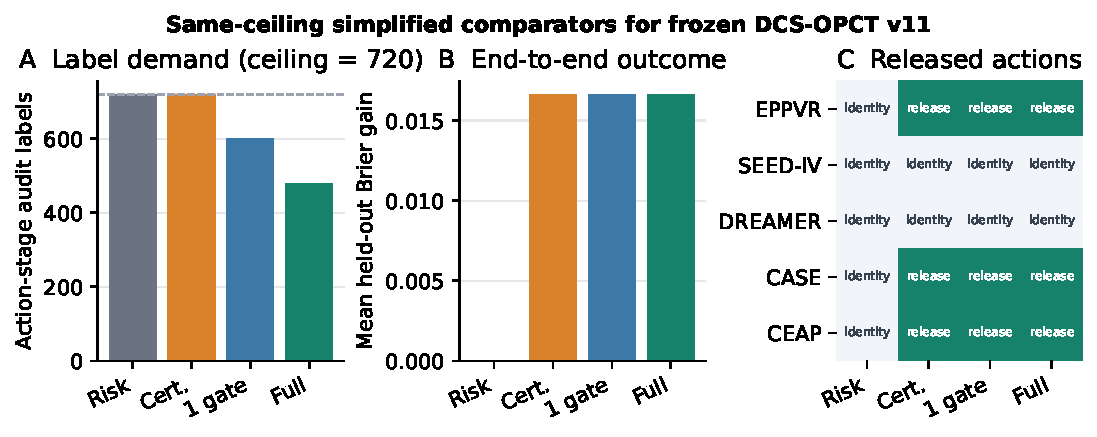
\includegraphics[width=\textwidth]{figures/fig_end_to_end_simplified_comparators.pdf}
\caption{Label demand, held-out outcome, and released actions for the simplified frozen variants. Identity in the risk-ranking-only column denotes that ranking does not itself define an intervention.}
\label{fig:supp-simplified-comparators}
\end{figure*}

\section{Post-hoc stability of frozen actions}

Eight frozen parameters were varied one at a time over two more permissive and two stricter local settings, yielding 320 domain--action rows. Every local relaxation preserved identity in DREAMER, SEED-IV, AVDOS-VR, FACED, and EEGEmotions-27. Four strict-setting rows changed a release: EPPVR failed only at directional agreement 0.95, whereas CEAP failed at directional agreement 0.95, displacement cosine 0.95, or Brier-gain lower bound 0.002. CASE did not flip. The complete three-level joint cube contained 6,561 scenarios and only three release patterns: EPPVR--CASE--CEAP, EPPVR--CASE, or CASE alone. This analysis maps local decision margins after freezing; it did not select thresholds or provide prospective effectiveness evidence.

\begin{table}[!htbp]
\centering
\caption{Frozen-action local stability summary. External-domain relaxation refers to AVDOS-VR, FACED, and EEGEmotions-27.}
\label{tab:frozen-action-stability}
\small
\begin{tabular}{lr}
\toprule
Diagnostic & Result \\
\midrule
One-at-a-time domain--action rows & 320 \\
Rows with an action flip & 4 \\
Domains affected by any local flip & EPPVR; CEAP \\
Joint local scenarios & 6,561 \\
Distinct release patterns & 3 \\
External domains released after relaxation & 0 \\
\bottomrule
\end{tabular}

\end{table}

\begin{figure*}[!htbp]
\centering
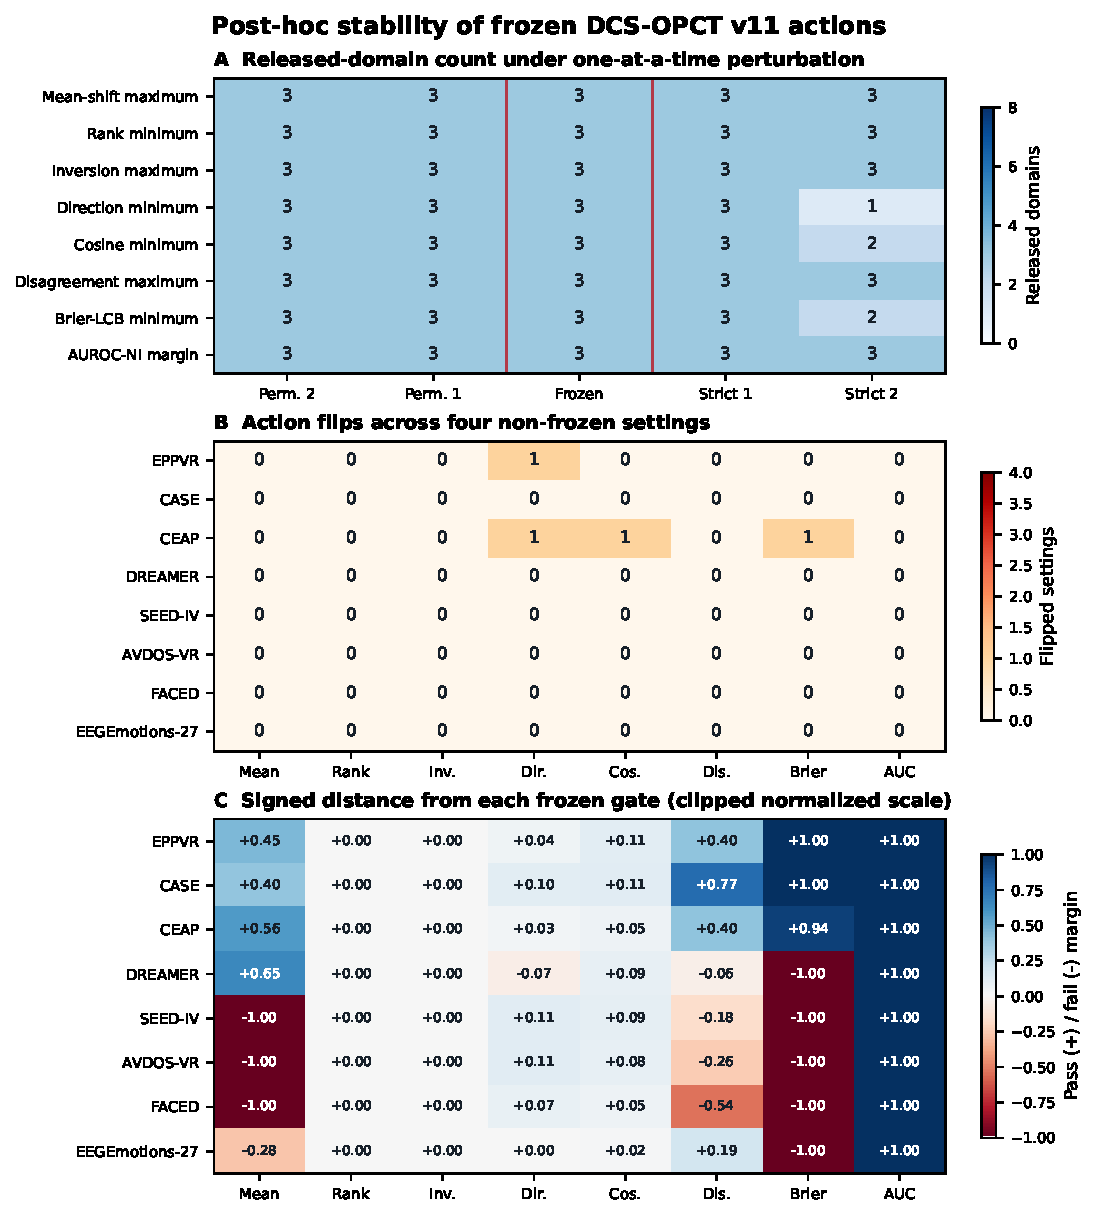
\includegraphics[width=0.88\textwidth]{figures/fig_frozen_action_stability.pdf}
\caption{Post-hoc local stability of the frozen DCS-OPCT v11 decisions. Positive signed margins pass a frozen gate and negative margins fail it. Rank and inversion margins are shown at their numerical boundary and should not be interpreted as substantive slack.}
\label{fig:frozen-action-stability}
\end{figure*}

\section{Worked frozen audit trace}

The EPPVR trace illustrates a released correction: the largest component shift was 0.055, directional agreement was 0.938, displacement cosine was 0.997, and normalized disagreement was 0.209. After both unlabeled stages passed, 160 action-stage labels entered the fixed audit. The one-sided Brier-gain lower bound was 0.0096, above the frozen 0.001 requirement, and the held-out gain was 0.0263. EEGEmotions-27 illustrates a pre-label stop: its largest component shift was 0.128, above 0.10, so the witness and labeled certificate were not reached and zero action-stage labels were accessed. Stages after a stop are marked N/A rather than shown as hypothetical passes. Identity is non-intervention and is not counted as effectiveness, non-harm, or successful external calibration.

\begin{figure*}[!htbp]
\centering
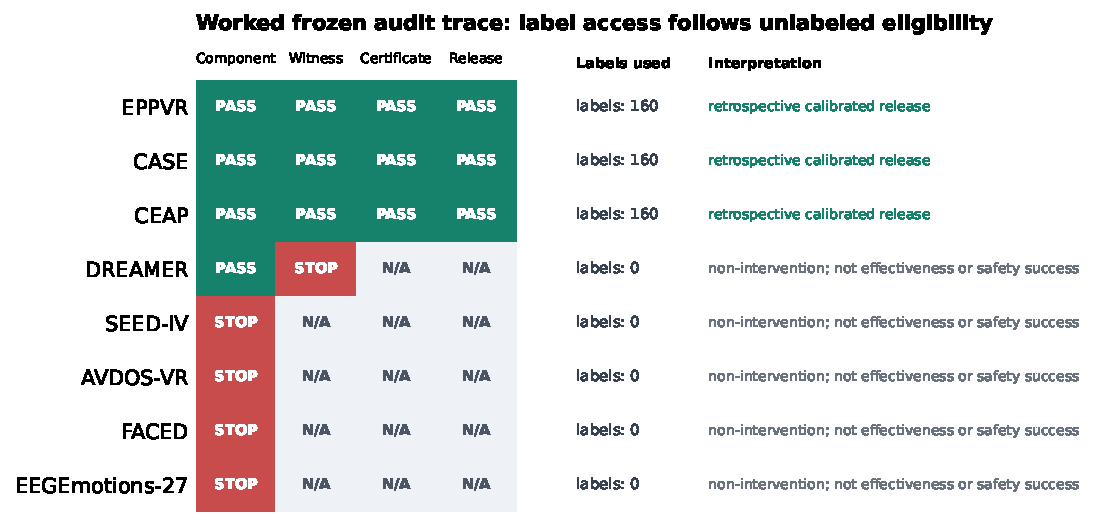
\includegraphics[width=0.92\textwidth]{figures/fig_worked_audit_trace.pdf}
\caption{Worked frozen action paths for a released development action (EPPVR) and a separate pre-signal external applicability failure (EEGEmotions-27).}
\label{fig:worked-audit-trace}
\end{figure*}

\section{Post-hoc seven-domain risk robustness}

We evaluated whether broadening the risk-model training pool was sufficient to remove cross-domain instability. The analysis retained the frozen 0.02 endpoint and the same five dataset-agnostic mechanism predictors. It combined 1,920 nonzero-dose subject-axis configurations from DEAP, MAHNOB-HCI, EPPVR, CASE, CEAP, SEED-IV, and DREAMER. Three L2 logistic models were compared: ordinary pooled fitting, equal total loss weight per training dataset, and a smooth worst-domain objective. All 147 nested fits used deterministic float64 CUDA optimization. For each outer held-out dataset, the operating threshold was selected exclusively from inner leave-one-dataset-out predictions over the six training domains.

The equal-domain model improved weighted Brier score from 0.1732 for the frozen two-source probabilities to 0.1621 and improved four of seven domains. Its five mechanism coefficients were positive in every outer fold (35 of 35 coefficients). This directional stability did not translate into reliable discrimination: median AUROC was 0.616, only four domains reached AUROC 0.60, and median balanced accuracy at the nested training-only threshold was 0.592. The prespecified gate required at least five domains at AUROC 0.60, median AUROC at least 0.65, and median balanced accuracy at least 0.60; all three conditions failed. CASE was the clearest boundary, with AUROC 0.468 and Brier skill $-0.096$ after equal-domain training. Nonlinear tree, histogram-gradient, and quadratic screening models were not promoted because none improved the overall leave-dataset-out result.

This analysis was specified only after the seven datasets had already been accessed, and its failed gate is retained. It therefore does not extend the prospective evidence level. Instead, it separates stable average mechanism direction from transportable risk ranking: adding heterogeneous source domains can reduce pooled probability error without yielding a common decision rule. This boundary motivates target-domain calibration and selective release but cannot itself validate DCS-OPCT.

\begin{center}
\begin{minipage}{\textwidth}
\refstepcounter{table}
\textbf{Table~\thetable:} Nested leave-one-dataset-out comparison of the frozen two-source v11 probability and the seven-domain equal-domain model. Prev. is endpoint prevalence; BS is Brier skill against the outer-fold training prevalence; BAcc uses a threshold selected only from inner training-domain predictions. The prespecified seven-domain robustness gate failed.
\label{tab:v12-multidomain}
\par\medskip
\centering
\small
\resizebox{\textwidth}{!}{\begin{tabular}{lrrrrrr}
\toprule
Dataset & Prev. & v11 AUROC & DB AUROC & v11 BS & DB BS & DB BAcc \\
\midrule
DEAP & 0.171 & 0.698 & 0.698 & 0.018 & 0.042 & 0.630 \\
MAHNOB-HCI & 0.304 & 0.735 & 0.735 & 0.069 & 0.070 & 0.686 \\
EPPVR & 0.163 & 0.666 & 0.667 & -0.128 & 0.023 & 0.619 \\
CASE & 0.209 & 0.471 & 0.468 & -0.378 & -0.096 & 0.454 \\
CEAP & 0.247 & 0.604 & 0.616 & -0.049 & 0.014 & 0.583 \\
SEED-IV & 0.058 & 0.557 & 0.540 & 0.367 & 0.179 & 0.592 \\
DREAMER & 0.292 & 0.586 & 0.581 & 0.011 & 0.018 & 0.544 \\
\bottomrule
\end{tabular}
}
\end{minipage}
\end{center}

\begin{figure}[!htbp]
\centering
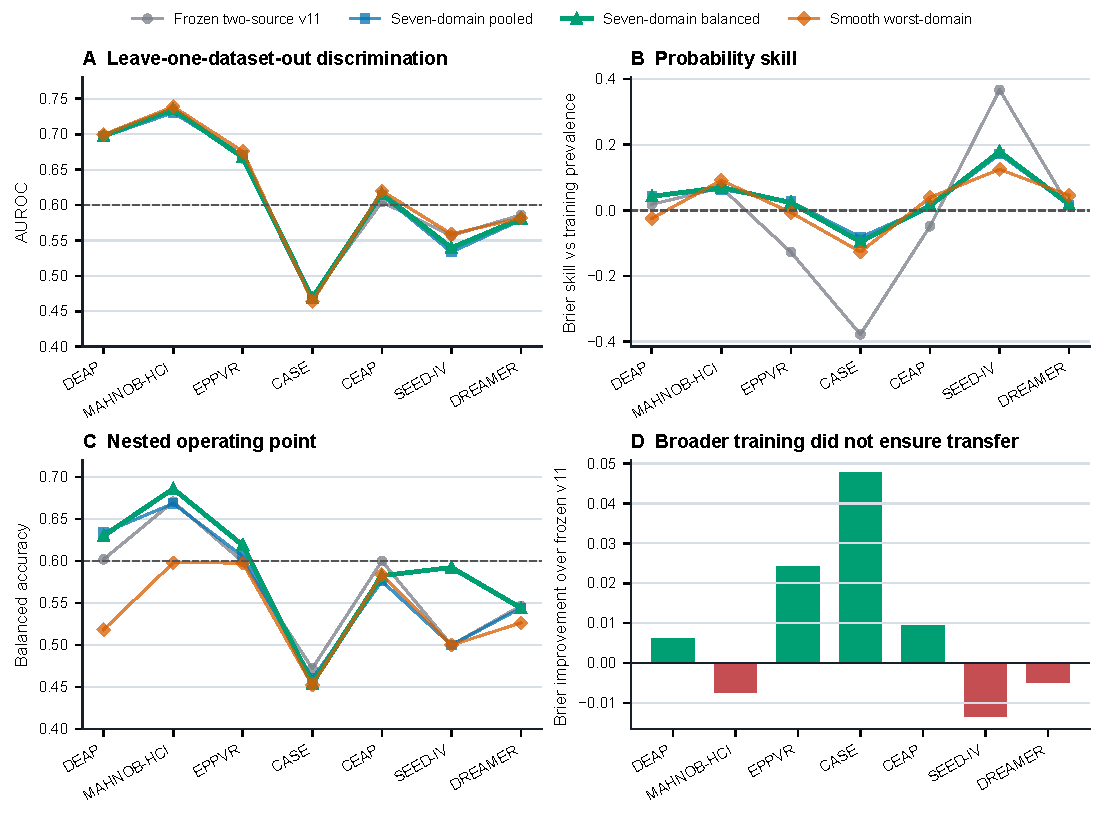
\includegraphics[width=\textwidth]{figures/fig_v12_multidomain_robustness.pdf}
\caption{Post-hoc seven-domain robustness analysis. (A) AUROC under nested leave-one-dataset-out evaluation; the dashed line is the prespecified 0.60 domain floor. (B) Brier skill against the outer-fold training prevalence. (C) Balanced accuracy at an operating threshold selected only from inner training-domain predictions; the dashed line is the 0.60 floor. (D) Brier-score improvement of the equal-domain model over the frozen two-source v11 probabilities; positive values favor broader training. The retrospective gate failed, so the figure diagnoses domain heterogeneity rather than external effectiveness.}
\label{fig:v12-multidomain}
\end{figure}


\section{EEGEmotions-27 pre-signal robustness boundary}

EEGEmotions-27 was pinned at repository commit \texttt{0dfec14d177e}; the complete commit identifier is retained in the registration and implementation lock. Registration followed inspection of the public README, channel metadata, and repository filenames, but preceded access to EEG sample values, participant demographics, derived features, predictions, or outcomes. The evidence role is therefore separate pre-signal robustness, not pristine prospective confirmation. The registered task maps fixed physical emotion-video categories to positive or negative polarity; it does not measure participant-experienced valence or arousal.

The structural analysis retained 87 participants and 864 participant--stimulus trials. The frozen grid produced 150 summary rows and 3,600 CUDA fitting units. The action and distribution-covered 15/15 audit--held-out cluster assignment were hashed before target outcomes entered the decision. CORAL plus OPCT shifted the mean probability by 0.1073 and quantile mapping plus OPCT by 0.1281; both exceeded the 0.10 applicability maximum. The witness and labeled certificate were therefore skipped and identity was retained.


\begin{table*}[t]
\centering
\caption{Post-outcome description of the frozen unlabeled applicability decision. Applicability itself was locked before target outcome labels were attached.}
\label{tab:eegemotions27-applicability}
\resizebox{\textwidth}{!}{%
\begin{tabular}{lrrrrrr}
\toprule
Projection & $|\Delta\bar p|$ & Limit & Excess & Rank & Inversions & Applicable \\
\midrule
CORAL + OPCT & 0.1073 & 0.10 & 0.0073 & 1.000000 & 0 & No \\
Quantile mapping + OPCT & 0.1281 & 0.10 & 0.0281 & 1.000000 & 0 & No \\
\bottomrule
\end{tabular}%
}
\end{table*}


\begin{table*}[t]
\centering
\caption{Descriptive dual-unseen category-polarity performance at zero identity dose. Mean $\pm$ SD summarizes five correlated frozen split seeds and is not an independent-sample confidence interval.}
\label{tab:eegemotions27-dual-generalization}
\resizebox{\textwidth}{!}{%
\begin{tabular}{llrrrr}
\toprule
Representation & Classifier & Seeds & Balanced accuracy & Range & Mean $-0.5$ \\
\midrule
All features & Logistic & 5 & 0.450 $\pm$ 0.051 & 0.365--0.493 & -0.050 \\
All features & GPU MLP & 5 & 0.422 $\pm$ 0.081 & 0.289--0.495 & -0.078 \\
Relative power & Logistic & 5 & 0.473 $\pm$ 0.042 & 0.398--0.499 & -0.027 \\
Relative power & GPU MLP & 5 & 0.413 $\pm$ 0.063 & 0.312--0.471 & -0.087 \\
Normalized asymmetry & Logistic & 5 & 0.458 $\pm$ 0.030 & 0.406--0.475 & -0.042 \\
Normalized asymmetry & GPU MLP & 5 & 0.400 $\pm$ 0.070 & 0.283--0.459 & -0.100 \\
\bottomrule
\end{tabular}%
}
\end{table*}


\begin{table*}[t]
\centering
\caption{Post-hoc encoding--utilization boundary. Identity margins are descriptive five-seed summaries. Event and ranking analyses cannot alter the frozen external gate.}
\label{tab:eegemotions27-boundary}
\begin{tabular}{llrr}
\toprule
Representation & Probe & Encoding margin & Range \\
\midrule
All features & Linear & 0.935 $\pm$ 0.005 & 0.928--0.942 \\
All features & RBF & 0.833 $\pm$ 0.008 & 0.826--0.846 \\
Relative power & Linear & 0.844 $\pm$ 0.005 & 0.837--0.850 \\
Relative power & RBF & 0.731 $\pm$ 0.007 & 0.722--0.740 \\
Normalized asymmetry & Linear & 0.819 $\pm$ 0.011 & 0.804--0.833 \\
Normalized asymmetry & RBF & 0.793 $\pm$ 0.012 & 0.772--0.804 \\
\bottomrule
\end{tabular}
\par\vspace{1.0ex}
\begin{tabular}{lr}
\toprule
Boundary diagnostic & Observed \\
\midrule
Audit material events & 4 positive, 1 negative \\ 
Held-out material events & 5 positive, 3 negative \\ 
Strong monotonic dose patterns & 0/30 \\ 
Model-ranking reversals & 6/60 \\ 
Representation-ranking reversals & 12/40 \\ 
\bottomrule
\end{tabular}
\end{table*}


\begin{figure*}[!htbp]
\centering
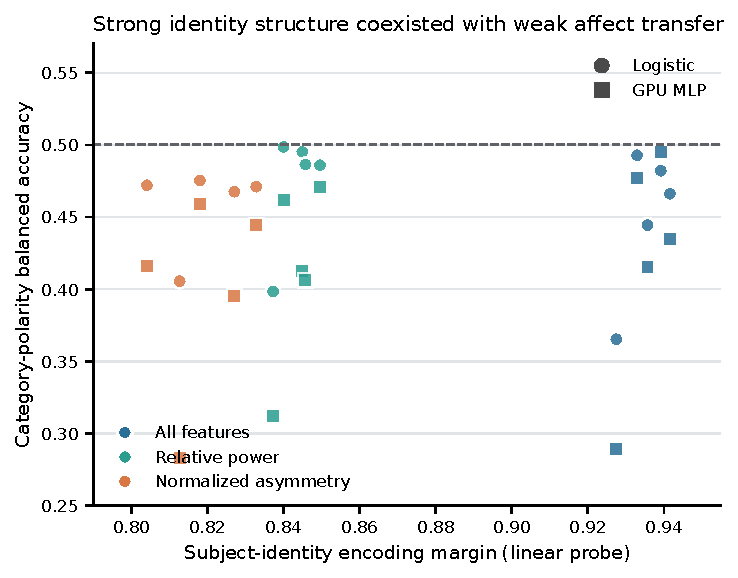
\includegraphics[width=0.78\textwidth]{figures/fig_eegemotions27_identity_vs_affect.pdf}
\caption{Post-hoc EEGEmotions-27 encoding--utilization boundary. Subject-identity encoding margins were high, while dual-unseen category-polarity balanced accuracy remained below chance on average for every representation--classifier combination. The figure is descriptive and cannot alter the frozen action.}
\label{fig:supp-eegemotions-identity}
\end{figure*}

\begin{figure*}[!htbp]
\centering
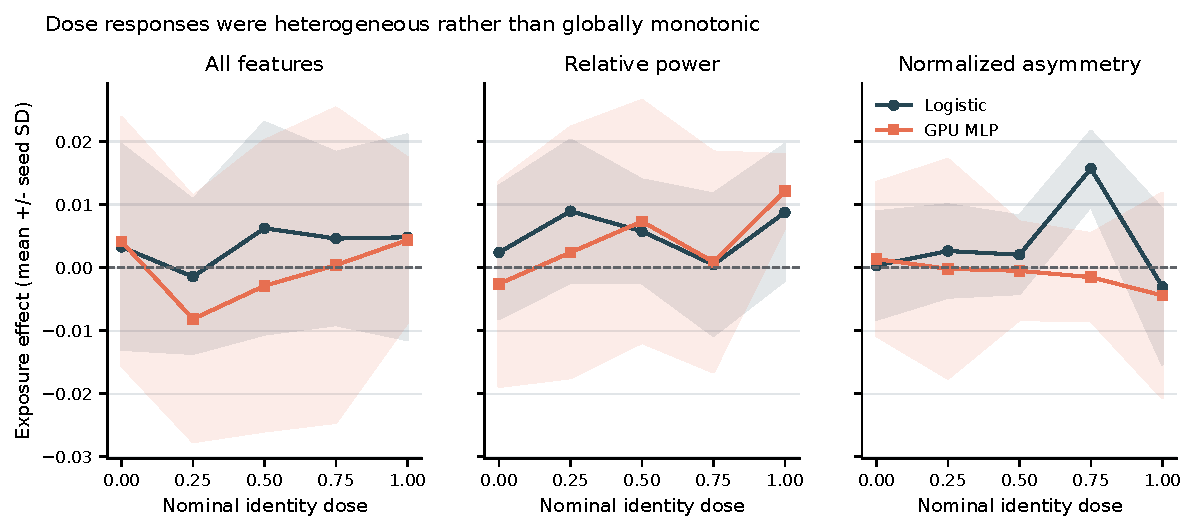
\includegraphics[width=\textwidth]{figures/fig_eegemotions27_dose_heterogeneity.pdf}
\caption{Post-hoc EEGEmotions-27 dose heterogeneity. Curves show mean exposure effects across five frozen seeds and shading shows one seed-level standard deviation. No evaluated configuration exhibited a strong globally monotonic dose pattern; these diagnostics explain heterogeneity but do not rescue the failed external gate.}
\label{fig:supp-eegemotions-dose}
\end{figure*}

The nonreleased held-out counterfactuals were unfavorable: CORAL plus OPCT had Brier gain $-0.0349$ and AUROC change $-0.0509$, while quantile mapping plus OPCT had Brier gain $-0.0569$ and AUROC change $-0.1200$. These values were unavailable to the pre-outcome applicability decision and are reported only to characterize the rejected actions. They cannot be used to retune the threshold or claim that abstention proved future-domain safety.

\section{EKM-ED prospective structural endpoint failure}

EKM-ED was reserved on 16 September 2026 before archive-member or participant-value access. Public Zenodo metadata identified 47 participants, a four-channel Muse S montage, four affective films plus baseline, 128-Hz clean signals, participant SAM ratings, and public key-moment timestamps. The official archive matched the registered byte count and MD5. A central-directory manifest was written without opening members, followed by a separately authorized header-only step that read exactly the first line of one deterministic SAM file and one deterministic clean-signal file. The schema-bound adapter and synthetic archive tests were then locked with the unchanged v11 risk model, five seeds, five doses, two classifiers, 40 CUDA epochs, and all release gates. The implementation-lock SHA-256 was \texttt{ec729f31\allowbreak{}62703381\allowbreak{}9af91368\allowbreak{}99508978\allowbreak{}0c2825da\allowbreak{}c3cee3f0\allowbreak{}ae233d73\allowbreak{}bf380235}.

The frozen endpoint used only TP9, AF7, AF8, and TP10 raw columns. Each participant--film aggregate required all three public key moments to provide complete finite 4-s windows, and each task required at least three retained films plus both SAM classes for every included participant. Table~\ref{tab:ekmed-structural-failure} reports the first and only confirmatory preparation attempt. No pre-outcome design lock, action lock, material-event outcome, or model fit was created.

\begin{table*}[!htbp]
\centering
\caption{Prospective EKM-ED structural audit under the frozen endpoint. Counts are participant--film units unless otherwise stated. Structural non-estimability cannot be interpreted as calibration failure, effectiveness, non-harm, or safety.}
\label{tab:ekmed-structural-failure}
\small
\setlength{\tabcolsep}{5pt}
\begin{tabular}{>{\raggedright\arraybackslash}p{0.29\textwidth}r>{\raggedright\arraybackslash}p{0.48\textwidth}}
\toprule
Audit item & Count & Interpretation \\
\midrule
Questionnaire participants attempted & 47 & All public questionnaire participants entered the locked attempt \\
Possible participant--film units & 188 & Four registered affective films per participant \\
Missing registered clean-signal file & 10 & Unit excluded before feature construction \\
Zero complete finite key-moment windows & 45 & Unit failed the three-window trial contract \\
One complete finite key-moment window & 47 & Unit failed the three-window trial contract \\
Retained three-window trials & 86 & Structurally valid trials before task-specific SAM filtering \\
Valence midpoint exclusions & 6 & Rating 5 removed by the frozen label rule \\
Arousal midpoint exclusions & 14 & Rating 5 removed by the frozen label rule \\
Eligible participants, valence & 0 & Minimum three trials and both classes not met \\
Eligible participants, arousal & 0 & Minimum three trials and both classes not met \\
\bottomrule
\end{tabular}
\end{table*}

The immutable failure record has SHA-256 \texttt{8f621780\allowbreak{}673a87e4\allowbreak{}55594ec4\allowbreak{}6e2bb38e\allowbreak{}f1538470\allowbreak{}f355471b\allowbreak{}46de0f64\allowbreak{}633cb070}. The confirmatory branch is final: changing key moments, alignment, completeness, labels, channels, or participant requirements after observing these counts would define an exploratory analysis and cannot overwrite this result. The failure locates an endpoint-transport boundary: semantically shared film events and a nominally compatible wearable montage did not guarantee enough complete participant-level trials for the frozen configuration-level risk endpoint.

\section{Covariate-unseen target-transform sensitivity}

The primary v11 analysis separated labels but allowed the complete unlabeled target configuration table to contribute to transformation fitting and distribution-covered assignment. We therefore constructed an explicitly inductive configuration-level sensitivity. Within every task--representation--model stratum, clusters were assigned from stratum labels and sorted split-seed identifiers only, alternating two and three audit seeds to preserve a balanced half split. This assignment did not read target features, candidate probabilities, or outcomes. CORAL covariance statistics, empirical quantile maps, positive-slope OPCT parameters, the component and witness gates, and the labeled certificate were estimated using the audit side only. The resulting frozen action was then applied once to covariate- and outcome-unseen held-out configurations.

\begin{table*}[!htbp]
\centering
\caption{Configuration-level inductive sensitivity. The transductive gain is the archived v11 outcome-held-out result. Identity actions have zero gain by construction and are non-interventions, not successful calibration.}
\label{tab:inductive-target}
\small
\setlength{\tabcolsep}{4pt}
\resizebox{\textwidth}{!}{%
\begin{tabular}{lccrrrl}
\toprule
Dataset & Components & Witness & Audit LCB & Inductive gain & Transductive gain & Inductive action \\
\midrule
EPPVR & pass & pass & 0.0152 & 0.0226 & 0.0263 & CORAL + OPCT \\
CASE & pass & pass & 0.0212 & 0.0406 & 0.0485 & CORAL + OPCT \\
CEAP & pass & fail & -- & 0.0000 & 0.0085 & identity \\
SEED-IV & fail & -- & -- & 0.0000 & 0.0000 & identity \\
DREAMER & pass & fail & -- & 0.0000 & 0.0000 & identity \\
\bottomrule
\end{tabular}
}
\end{table*}

Both released inductive actions had positive held-out Brier gain, zero AUROC change, and no material negative-transfer event. The result supports EPPVR and CASE under a stronger information-access protocol and identifies CEAP as target-batch dependent. It does not establish participant- or stimulus-level independence: configurations indexed by different split seeds can still reuse underlying observations. The analysis and its independent validator preserve this limitation explicitly; validation passed 12/12 checks.

\section{Raw test-group independence sensitivity}

The configuration-level inductive split still allows endpoint estimates from different split seeds to reuse the same test participants and physical stimuli. We therefore reconstructed separate endpoint labels before applying the inductive action protocol. Sorted participant identifiers were alternated into audit and evaluation sets. CASE, CEAP, SEED-IV, and DREAMER additionally used alternating verified physical-stimulus sets; audit labels were calculated only on the audit-participant--audit-stimulus diagonal and evaluation labels only on the disjoint evaluation diagonal. EPPVR used participant-disjoint rows because trial position is not a verified cross-participant physical-stimulus identifier. Dose and dose-zero predictions were paired by raw row identifier within each subset, and both classes were required in every evaluated cell.

\begin{table*}[!htbp]
\centering
\caption{Nested configuration- and raw-test-group independence sensitivity. Return-original actions have zero gain by construction and do not demonstrate calibration effectiveness.}
\label{tab:raw-group-independence}
\small
\resizebox{\textwidth}{!}{%
\begin{tabular}{lccrrrrl}
\toprule
Dataset & Components & Witness & Audit event rate & Evaluation event rate & Audit LCB & Evaluation gain & Action \\
\midrule
EPPVR & pass & pass & 0.1563 & 0.3000 & 0.0254 & 0.0135 & CORAL + OPCT \\
CASE & pass & pass & 0.3625 & 0.3063 & $-0.0091$ & 0.0000 & return original \\
CEAP & pass & fail & 0.3625 & 0.4813 & -- & 0.0000 & return original \\
SEED-IV & fail & -- & 0.1083 & 0.1500 & -- & 0.0000 & return original \\
DREAMER & pass & fail & 0.4333 & 0.2333 & -- & 0.0000 & return original \\
\bottomrule
\end{tabular}%
}
\end{table*}

Only EPPVR retained a released action, with positive participant-disjoint evaluation gain and zero AUROC change. CASE illustrates why configuration-level separation alone is insufficient: its action was positive in the covariate-unseen sensitivity, but the certificate failed once audit labels were reconstructed from a disjoint raw participant--stimulus subset. The analysis passed 13/13 independent validation checks. It removes overlap in raw test participants and, where identifiable, physical stimuli; it does not retrain the emotion models on disjoint training populations, and model-training rows and repeated split-seed fits can remain shared. It is therefore a stronger dependence sensitivity, not a fully independent external replication.

\section{Raw-partition-first EPPVR sensitivity}

To remove the remaining model-training dependence, we assigned the 30 EPPVR participants to two 15-person populations by lexicographic subject-identifier parity. No feature, label, endpoint, or model output entered this assignment. Within each population, the complete subject-axis experiment was rebuilt independently: two affective tasks, four representations, two model families, five split seeds, five subject folds, two within-subject record folds, and five identity-opportunity doses. This produced 4,800 emotion-model fits per population, or 9,600 total; all MLP fits used CUDA for 40 epochs. Identity encoding was also re-estimated separately with 80 probe fits per population. A 9,760-row provenance ledger records the population, train and test participant sets, global-row-set hashes, and zero row overlap for every fitted model.

Each population produced 320 nonzero-dose audit-risk configurations. The audit population alone was used to estimate CORAL covariance statistics, marginal quantile maps, positive-slope OPCT parameters, component and witness gates, outcome-blind distribution-covered assignment, and the 160-configuration release certificate. No evaluation-population covariate, endpoint, raw row, or fitted emotion model entered these operations. The locked release-or-return-original action was then applied once to all 320 evaluation-population configurations.

\begin{table*}[t]
\centering
\caption{Independence ladder for the DCS-OPCT development evidence. Return original denotes non-intervention, not successful calibration.}
\label{tab:independence-ladder}
\footnotesize
\resizebox{\textwidth}{!}{%
\begin{tabular}{lllllr}
\toprule
Protocol & Evaluation covariates & Endpoint raw groups & Emotion-model training & Released domains & EPPVR gain \\
\midrule
Transductive outcome holdout & Complete target batch used & Shared underlying observations & Shared & EPPVR, CASE, CEAP & 0.0263 \\
Covariate-unseen & Evaluation side unseen & Shared underlying observations & Shared & EPPVR, CASE & 0.0226 \\
Raw test-group separation & Evaluation side unseen & Disjoint test participants & Shared & EPPVR & 0.0135 \\
Raw partition first & Evaluation population unseen & Disjoint participants and rows & Disjoint & None; applicability stop & 0.0000 \\
\bottomrule
\end{tabular}%
}
\end{table*}


Audit- and evaluation-population event prevalence was 0.2219 (71/320) and 0.2719 (87/320), respectively. The frozen risk model overpredicted absolute event frequency in both populations: mean probabilities were 0.4504 and 0.5527. More importantly, the audit-fitted CORAL and quantile OPCT components required mean shifts of $-0.2122$ and $-0.2030$. Both preserved rank exactly and had zero order inversions, but both violated the frozen absolute mean-shift limit of 0.10. The component screen therefore declared the target batch inapplicable; the witness and labeled certificate were not used to release a correction, and all evaluation configurations retained the original probabilities. Evaluation gain and AUROC change are consequently zero by construction.

The independent validator passed 21/21 checks, including exact fit counts, 15/15 participant separation, disjoint participant sets, population-contained prediction and training rows, zero train--test row overlap in every fit, complete 320-configuration risk tables, audit-only component fitting, and release/certificate consistency. The result closes the specific shared-training-row objection for EPPVR but does not provide positive calibration evidence: it shows that the earlier EPPVR release depends on a larger or less strictly partitioned target batch. Because this is one retrospective split of one dataset, it is not a new-dataset external validation, a cross-session test, a stimulus-independent test, or an estimate of future-domain performance. The unreleased candidate's evaluation behavior was not used to alter the frozen 0.10 limit.

\section{Endpoint measurement-error sensitivity}

The frozen endpoint thresholds the paired dose-induced balanced-accuracy amplification at 0.02. To quantify uncertainty in that estimated amplification, we applied 5,000 paired multinomial bootstrap draws to the underlying test predictions. Participant and physical-stimulus weights were crossed and held common between each nonzero-dose condition and its dose-zero anchor. This reconstructs the archived point amplification to numerical tolerance while propagating finite test-sample variation. It does not propagate repeated model-fitting variation or dependence induced by shared training rows across configurations.

\begin{table*}[!htbp]
\centering
\caption{Crossed test-sample uncertainty for the frozen source endpoint. CI crossing counts configurations whose 95\% bootstrap interval includes 0.02; LCB events require the lower bound to reach 0.02.}
\label{tab:endpoint-uncertainty-source}
\small
\resizebox{\textwidth}{!}{%
\begin{tabular}{lrrrrr}
\toprule
Dataset & Configurations & Hard events & CI crossing & LCB events & Median $\Pr(A\geq0.02)$ \\
\midrule
DEAP & 240 & 41 & 238 & 0 & 0.2890 \\
MAHNOB-HCI & 240 & 73 & 240 & 0 & 0.3365 \\
\bottomrule
\end{tabular}%
}
\end{table*}

We then refitted the same L2-logistic form using $\Pr(A_{c,d}\geq0.02)$ as a soft target. When DEAP was held out, soft-label Brier score improved from 0.04345 for the frozen hard-label model to 0.03502 for the probabilistic-label model; when MAHNOB-HCI was held out, it improved from 0.06079 to 0.05724. Hard-label AUROC decreased from 0.69984 to 0.68256 and from 0.75228 to 0.70946, respectively. Prediction Spearman correlations between the hard- and soft-label models were 0.908 and 0.714. Several coefficient signs differed across the two transfers, so coefficient direction is not claimed to be stable after measurement-error propagation.

The same soft-event construction was applied to the five retrospective target-development domains. EPPVR used participant-only resampling because its records do not contain a verified cross-participant physical-stimulus identifier; the other domains used crossed participant and stimulus weights. Table~\ref{tab:endpoint-uncertainty-actions} evaluates the already frozen inductive actions against these soft labels. No action was reselected using the soft endpoint.

\begin{table*}[!htbp]
\centering
\caption{Post-hoc soft-endpoint evaluation of frozen inductive actions. Positive gain favors the released action; zero denotes a return-original action and is not evidence of calibration effectiveness.}
\label{tab:endpoint-uncertainty-actions}
\small
\resizebox{\textwidth}{!}{%
\begin{tabular}{lrrrrl}
\toprule
Dataset & Held-out $n$ & Hard prevalence & Soft prevalence & Soft Brier gain & Frozen action \\
\midrule
EPPVR & 160 & 0.1688 & 0.2437 & 0.0161 & released \\
CASE & 160 & 0.2125 & 0.3139 & 0.0209 & released \\
CEAP & 160 & 0.2938 & 0.3890 & 0.0000 & return original \\
SEED-IV & 120 & 0.0583 & 0.1914 & 0.0000 & return original \\
DREAMER & 120 & 0.2833 & 0.3705 & 0.0000 & return original \\
\bottomrule
\end{tabular}%
}
\end{table*}

The maximum point-reconstruction discrepancy was $2.85\times10^{-16}$. Independent validation passed 12/12 checks for source endpoint propagation and 12/12 checks for target action propagation. These results support only robustness of the direction of the two released actions to a probabilistic endpoint; they simultaneously show that hard event counts and mechanism-coefficient interpretation are highly sensitive to finite test-sample uncertainty.

\section{Nearest-neighbor baselines}

We adapted one covariate-shift calibration method and one unlabeled target-performance estimator to the configuration-level audit-risk task. The CPCS-style candidate estimated source importance weights with a balanced source-versus-target domain discriminator, using source configuration labels and audit-side unlabeled target features. Weights were odds-corrected for source/target sample size, clipped before normalization, and used to fit a positive-slope weighted Platt map on source endpoint labels. The target audit labels were reserved for the same 5,000-bootstrap release certificate used by inductive DCS-OPCT. Thus, both methods used the same target audit-label count, while CPCS-style fitting additionally used source labels and no target fitting labels.

\begin{table*}[!htbp]
\centering
\caption{Full-budget inductive DCS-OPCT versus the CPCS-style source-weighted candidate. CPCS gain is zero because every candidate failed the common certificate and returned the original probability.}
\label{tab:cpcs-style}
\small
\resizebox{\textwidth}{!}{%
\begin{tabular}{lrrrrrr}
\toprule
Dataset & Audit labels & CPCS audit gain & CPCS LCB & CPCS release & CPCS gain & DCS gain \\
\midrule
EPPVR & 160 & $-0.0196$ & $-0.0268$ & no & 0.0000 & 0.0226 \\
CASE & 160 & $-0.0136$ & $-0.0178$ & no & 0.0000 & 0.0406 \\
CEAP & 160 & $-0.0056$ & $-0.0099$ & no & 0.0000 & 0.0000 \\
SEED-IV & 120 & $-0.0019$ & $-0.0063$ & no & 0.0000 & 0.0000 \\
DREAMER & 120 & $-0.0043$ & $-0.0082$ & no & 0.0000 & 0.0000 \\
\bottomrule
\end{tabular}%
}
\end{table*}

The domain-discriminator AUROC ranged from 0.849 to 1.000, indicating substantial covariate separation rather than a benign shift. Effective source sample sizes after weighting ranged from 43.7 to 145.6 of 480 configurations. The uniformly negative certificates provide an empirical failure instance for source-weighted calibration under the present configuration-level endpoint, not a claim that CPCS fails generally. TransCal was not forced into this table because its primary object is confidence from a target-adapted task classifier; the present pipeline retains one unchanged audit-risk classifier and has no target-adapted classifier logits. A nominal implementation would therefore change both the input object and resource contract rather than supply a matched comparator.

The ATC-style analysis retained its native aggregate output. The source confidence threshold was 0.6763 and matched source hard-classification accuracy 0.7792. Table~\ref{tab:atc-style} compares unlabeled target accuracy estimates with observed inductive held-out accuracy. No probability correction or release was constructed from these estimates.

\begin{table*}[!htbp]
\centering
\caption{ATC-style aggregate accuracy estimation. Error is absolute estimated minus observed hard-classification accuracy. Brier gain and material-negative release are not defined because ATC does not output corrected configuration probabilities.}
\label{tab:atc-style}
\small
\begin{tabular}{lrrr}
\toprule
Dataset & Estimated accuracy & Observed accuracy & Absolute error \\
\midrule
EPPVR & 0.6938 & 0.7250 & 0.0313 \\
CASE & 0.6938 & 0.6625 & 0.0313 \\
CEAP & 0.7813 & 0.6938 & 0.0875 \\
SEED-IV & 1.0000 & 0.9417 & 0.0583 \\
DREAMER & 0.8500 & 0.7250 & 0.1250 \\
\bottomrule
\end{tabular}
\end{table*}

Independent validation passed 14/14 checks, including candidate resource accounting, equality of target audit-label budgets, positive calibration slopes, bounded weight ratios, return-original behavior, and the non-interventional ATC output contract.


\section{Evidence-role matrix}

Table~\ref{tab:evidence-role-matrix} separates empirical evidence from protocol readiness. AMIGOS and Emognition are not counted as completed experiments, EEGEmotions-27 is not promoted into that prospective family, and EKM-ED is counted as a completed prospective attempt but not as an effectiveness experiment because it failed before model fitting. This organization prevents dataset count from being used as a surrogate for evidential independence.

\begin{table*}[!htbp]
\centering
\caption{Evidence roles and inferential boundaries. Original dataset licenses, approvals, and participant-consent conditions govern data release.}
\label{tab:evidence-role-matrix}
\small
\setlength{\tabcolsep}{3pt}
\renewcommand{\arraystretch}{1.08}
\begin{tabular}{@{}>{\raggedright\arraybackslash}p{0.15\textwidth}>{\raggedright\arraybackslash}p{0.19\textwidth}>{\raggedright\arraybackslash}p{0.23\textwidth}>{\raggedright\arraybackslash}p{0.29\textwidth}@{}}
\toprule
Evidence layer & Datasets & Empirical contribution & Claim boundary \\
\midrule
Mechanism sources & DEAP; MAHNOB-HCI & Dose experiment and frozen risk-model training & Source-domain development, not external confirmation \\
Target development & EPPVR; CASE; CEAP; SEED-IV; DREAMER & Calibration release or identity fallback under the frozen action & Same-study retrospective evidence; no prospective effectiveness claim \\
Post-access tests & AVDOS-VR; FACED & Cross-physiology and common-montage failure boundaries & Non-intervention or non-estimability, not effectiveness or safety success \\
Pre-signal test & EEGEmotions-27 & Applicability failure before action-stage label access & Outside the prospective family; category polarity is not experienced affect \\
Prospective structural test & EKM-ED & Checksum-verified, implementation-locked endpoint construction attempted once & Zero eligible participants; no model fit, action, effectiveness, non-harm, or safety result \\
Reserved tests & AMIGOS; Emognition & Locked access, schema, GPU, and one-shot execution stacks & No result yet; both independent tests are still required \\
\bottomrule
\end{tabular}

\end{table*}

\section{Reproducibility and claim boundary}

The frozen model, v11 protocol, development script, input tables, assignments, and output manifests are linked by SHA-256 checksums. Independent validation passed 9 of 9 development checks, 17 of 17 leave-one-component checks, 17 of 17 seven-domain robustness checks, 11 of 11 seven-domain artifact checks, 12 of 12 AVDOS exploratory checks, 18 of 18 FACED exploratory checks, 12 of 12 EEGEmotions-27 one-shot checks, 6 of 6 EEGEmotions-27 post-hoc artifact checks, 13 of 13 simplified-comparator checks, 14 of 14 frozen-action-stability checks, 12 of 12 worked-example checks, 16 of 16 complete-cluster audit-yield checks, 8 of 8 cluster-score aggregation checks, 21 of 21 raw-partition-first checks, and 78 of 78 submission-artifact checks. The EKM-ED chain adds an 8/8 pre-member stack, an exact archive checksum, central-directory and header-only receipts, seven implementation-lock tests, a schema-bound implementation lock, and the immutable structural-failure record. The release-readiness driver additionally refreshes the 13-group AMIGOS and 15-group Emognition pre-access CUDA stacks and verifies that both reports hash the current implementation-lock, one-shot, and end-to-end test code. The Emognition stack includes separate field-level and ZIP-level fail-closed adapter tests. A dataset-level availability matrix records provider-controlled inputs, releasable derivatives, evidence roles, and claim boundaries. A separate non-self-referential reproducibility inventory hashes the readiness driver and report, both pre-access stack reports, the complete frozen-artifact inventory, reviewer-closure analyses, submission manifest and validation report, and the manuscript and supplementary TEX/PDF files; an independent validator checks every recorded byte count and digest. These checks establish internal reproducibility and pre-access software readiness; they do not substitute for external effectiveness confirmation.

The current reproducibility inventory contains 264 files and passed 23/23 checks. The consolidated reviewer-closure validator passed 14/14 checks. The release-readiness driver passed 6/6 gates, including the fail-closed external-arrival detector, whose own validation passed 7/7. AMIGOS and Emognition remained blocked by external data access. The checksum-verified EKM-ED implementation lock and structural-failure record are included in the current non-overwriting inventory and submission package; their existence does not convert structural non-estimability into effectiveness or future-domain non-harm evidence.

\begin{itemize}
\setlength{\itemsep}{1pt}
\setlength{\parskip}{0pt}
\setlength{\parsep}{0pt}
\item The transported endpoint is configuration-level material identity optimism.
\item DCS-OPCT does not change EEG emotion-classifier predictions or accuracy.
\item Identity fallback demonstrates non-intervention, not effectiveness.
\item AVDOS-VR is post-access exploratory evidence only.
\item FACED is post-access exploratory evidence only; the registered 32-channel branch was structurally ineligible.
\item EEGEmotions-27 is a separate pre-signal robustness test outside the AMIGOS/Emognition prospective family; category polarity is stimulus-derived and the identity result is not effectiveness or safety success.
\item EKM-ED is a completed prospectively locked attempt whose frozen endpoint was structurally ineligible before model fitting; it is not an effectiveness, non-harm, or safety result.
\item An event-free endpoint makes calibration effectiveness non-estimable rather than successful.
\item No universal prevention of negative transfer is claimed.
\item A positive external-effectiveness claim still requires a compatible prospectively reserved dataset that passes the unchanged endpoint, action, audit, and held-out gates.
\end{itemize}

\begin{figure*}[!htbp]
\centering
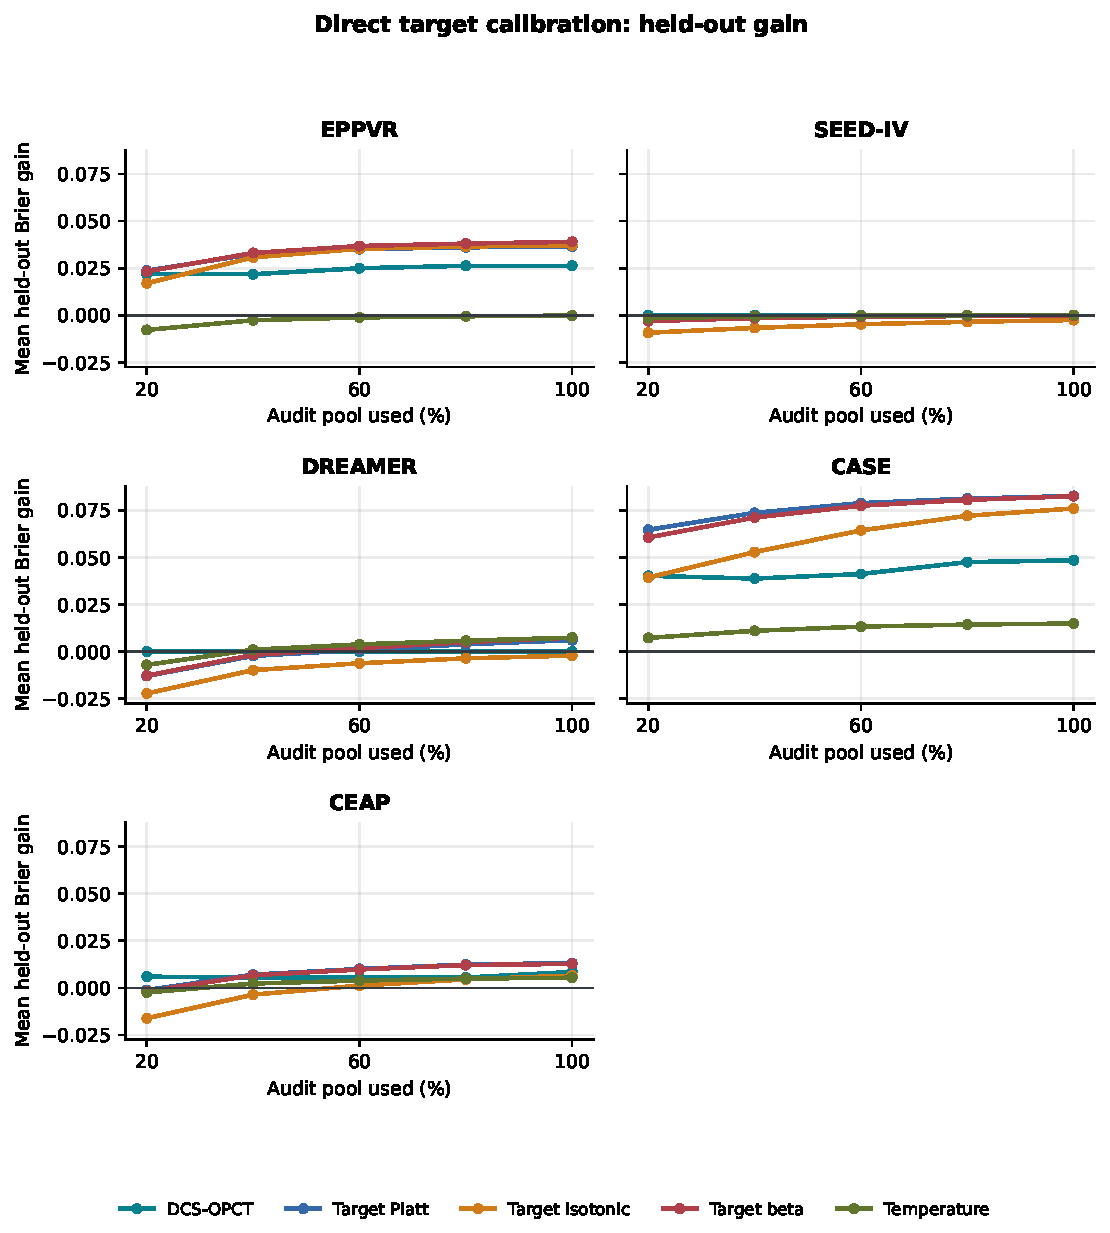
\includegraphics[width=\textwidth]{figures/fig_direct_calibration_gain_readable.pdf}
\caption{Dataset-specific held-out Brier gain for selective DCS-OPCT and direct target-label calibrators.}
\label{fig:direct-gain-readable}
\end{figure*}

\begin{figure*}[!htbp]
\centering
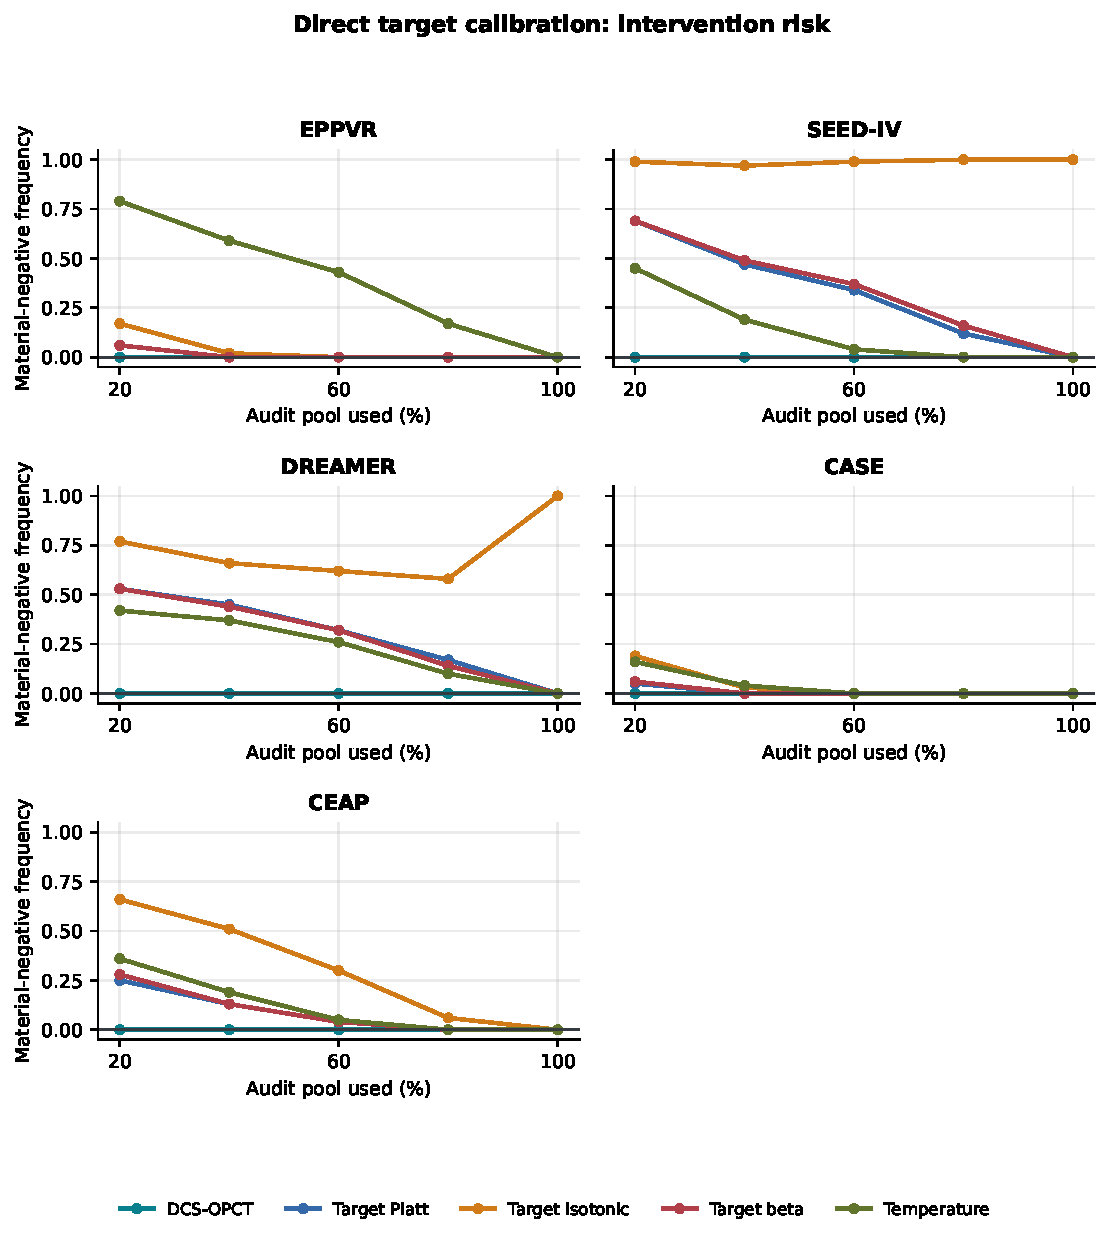
\includegraphics[width=\textwidth]{figures/fig_direct_calibration_risk_readable.pdf}
\caption{Material-negative-transfer frequency for direct target calibration. Identity fallback in DCS-OPCT is non-intervention, not effectiveness. Curves are retrospective sensitivity results on fixed held-out halves.}
\label{fig:direct-risk-readable}
\end{figure*}

\begin{figure*}[!htbp]
\centering
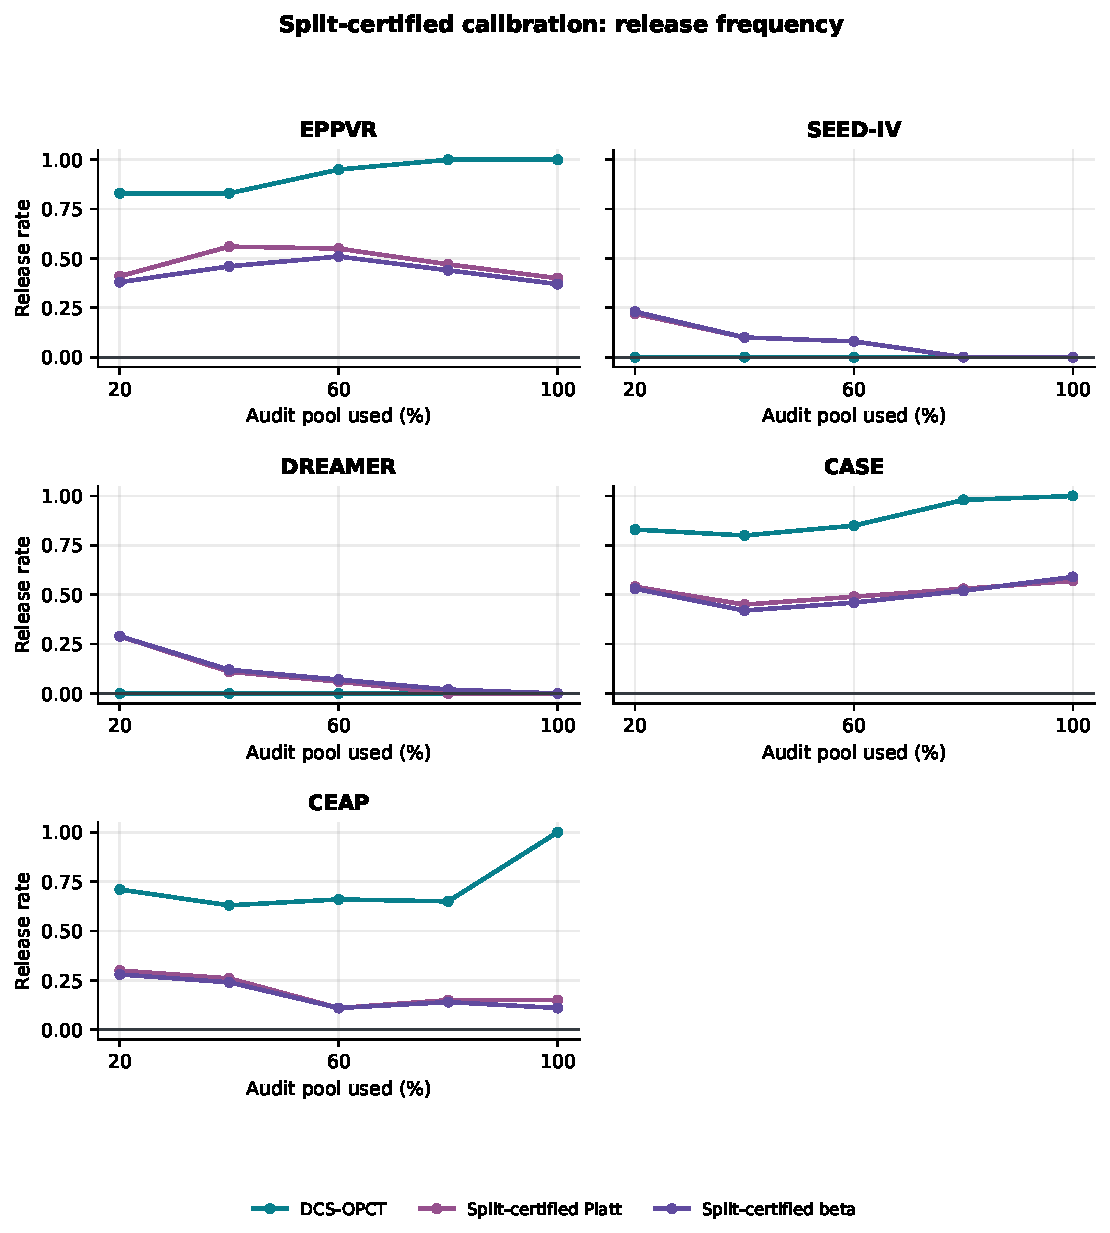
\includegraphics[width=\textwidth]{figures/fig_split_certified_release_readable.pdf}
\caption{Release frequency for selective DCS-OPCT and split-fit/certified Platt or monotone beta calibration.}
\label{fig:split-release-readable}
\end{figure*}

\begin{figure*}[!htbp]
\centering
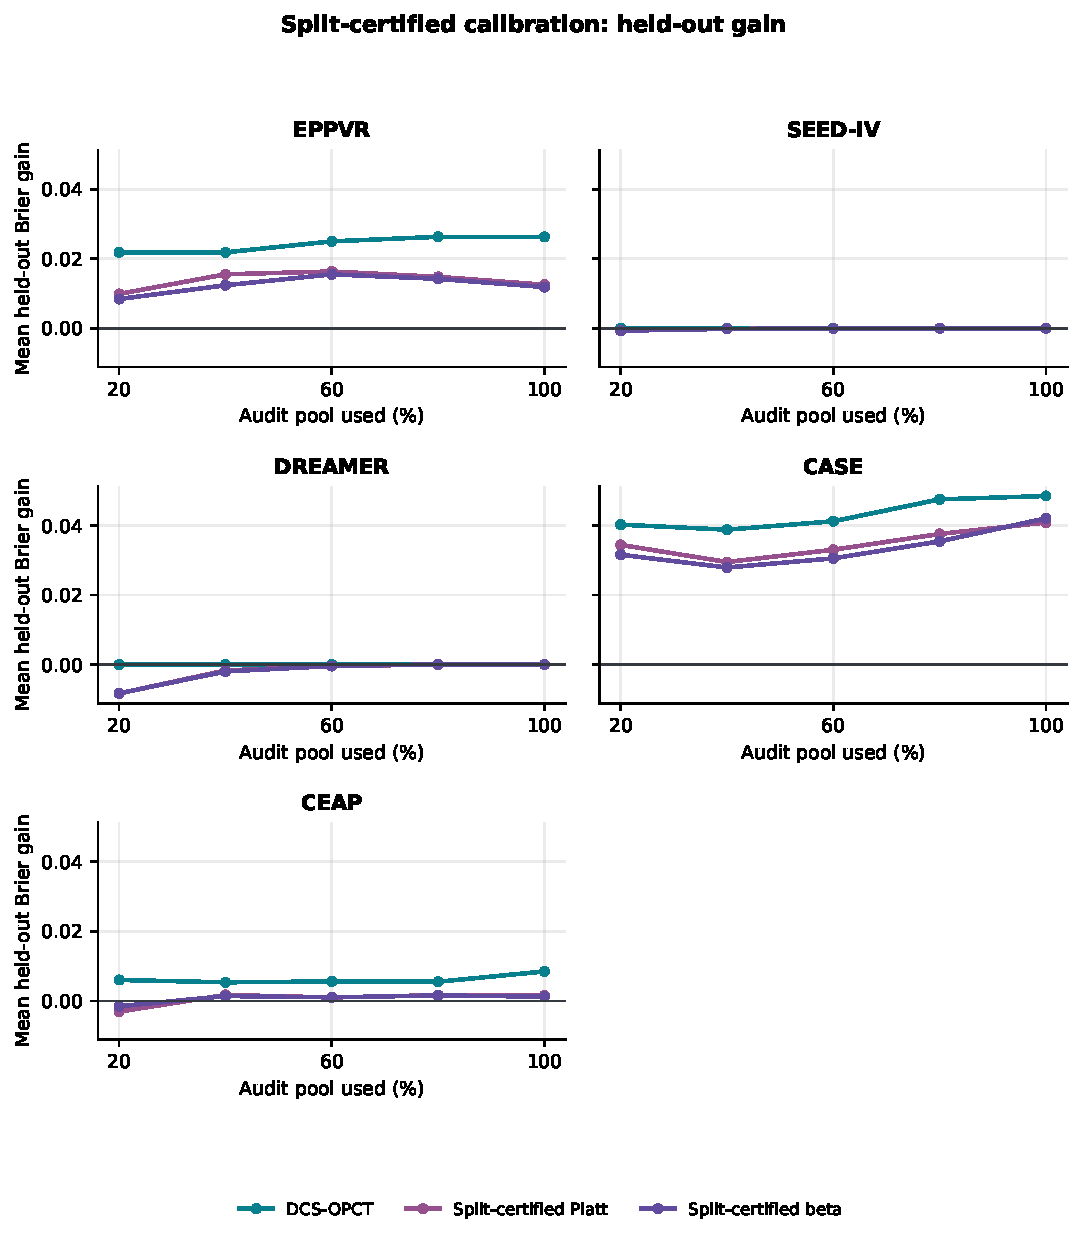
\includegraphics[width=\textwidth]{figures/fig_split_certified_gain_readable.pdf}
\caption{Held-out Brier gain for selective DCS-OPCT and split-fit/certified calibration. Rejected repetitions contribute identity gain zero.}
\label{fig:split-gain-readable}
\end{figure*}

\begin{figure*}[!htbp]
\centering
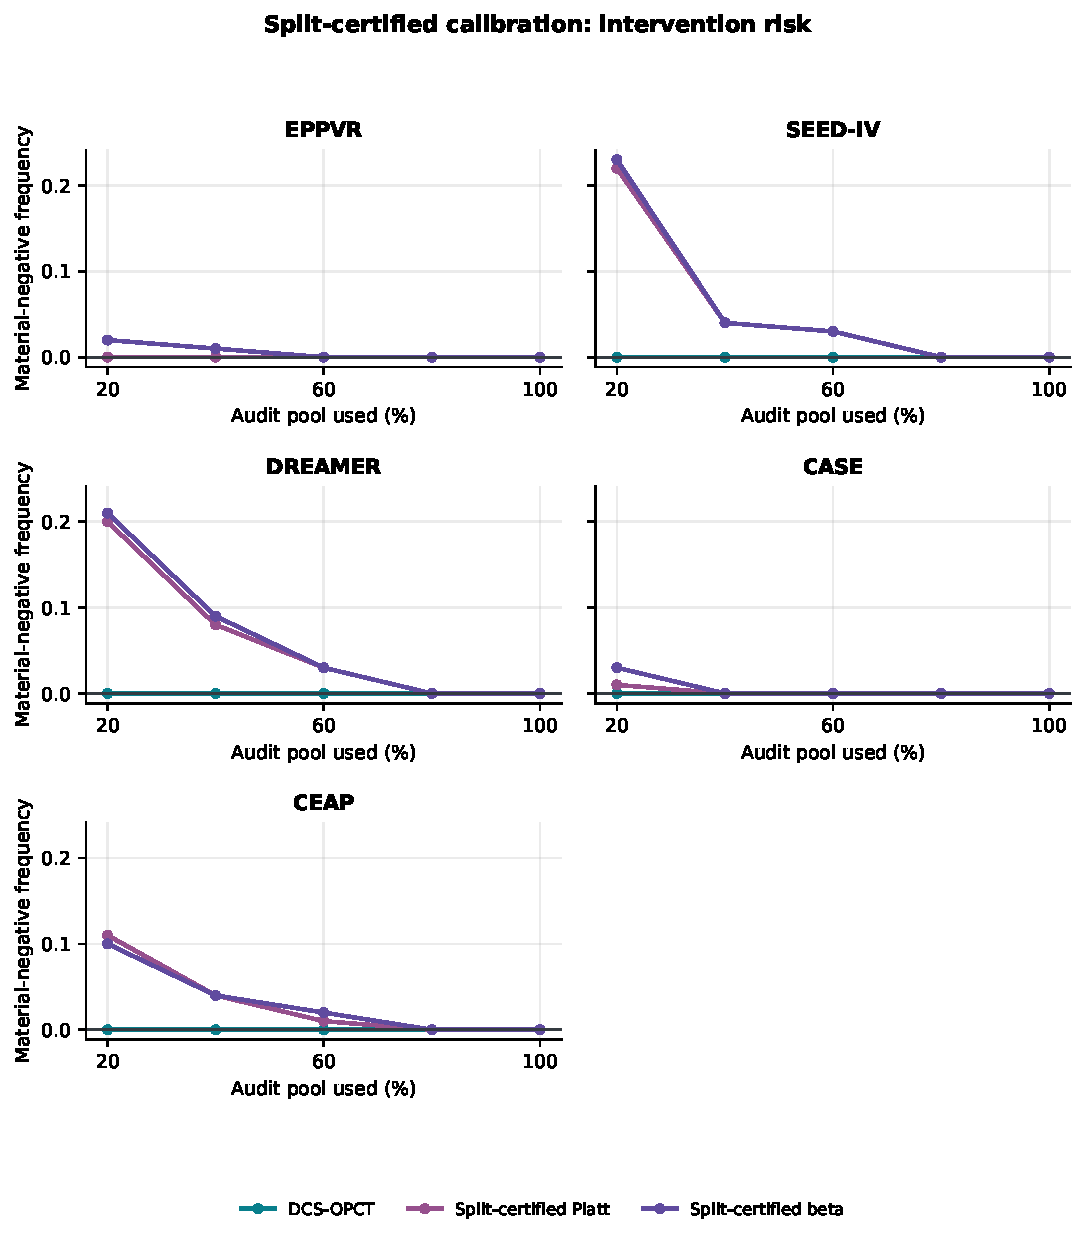
\includegraphics[width=\textwidth]{figures/fig_split_certified_risk_readable.pdf}
\caption{Material-negative-transfer frequency for selective DCS-OPCT and split-fit/certified calibration. Corresponding 20\% budget paired inference is reported in Table~\ref{tab:crossfit-paired}.}
\label{fig:split-risk-readable}
\end{figure*}

\end{document}
